\chapter{Implementation}

\section{Google Cloud Platform (GCP)}
\subsection{GCP Dashboard}
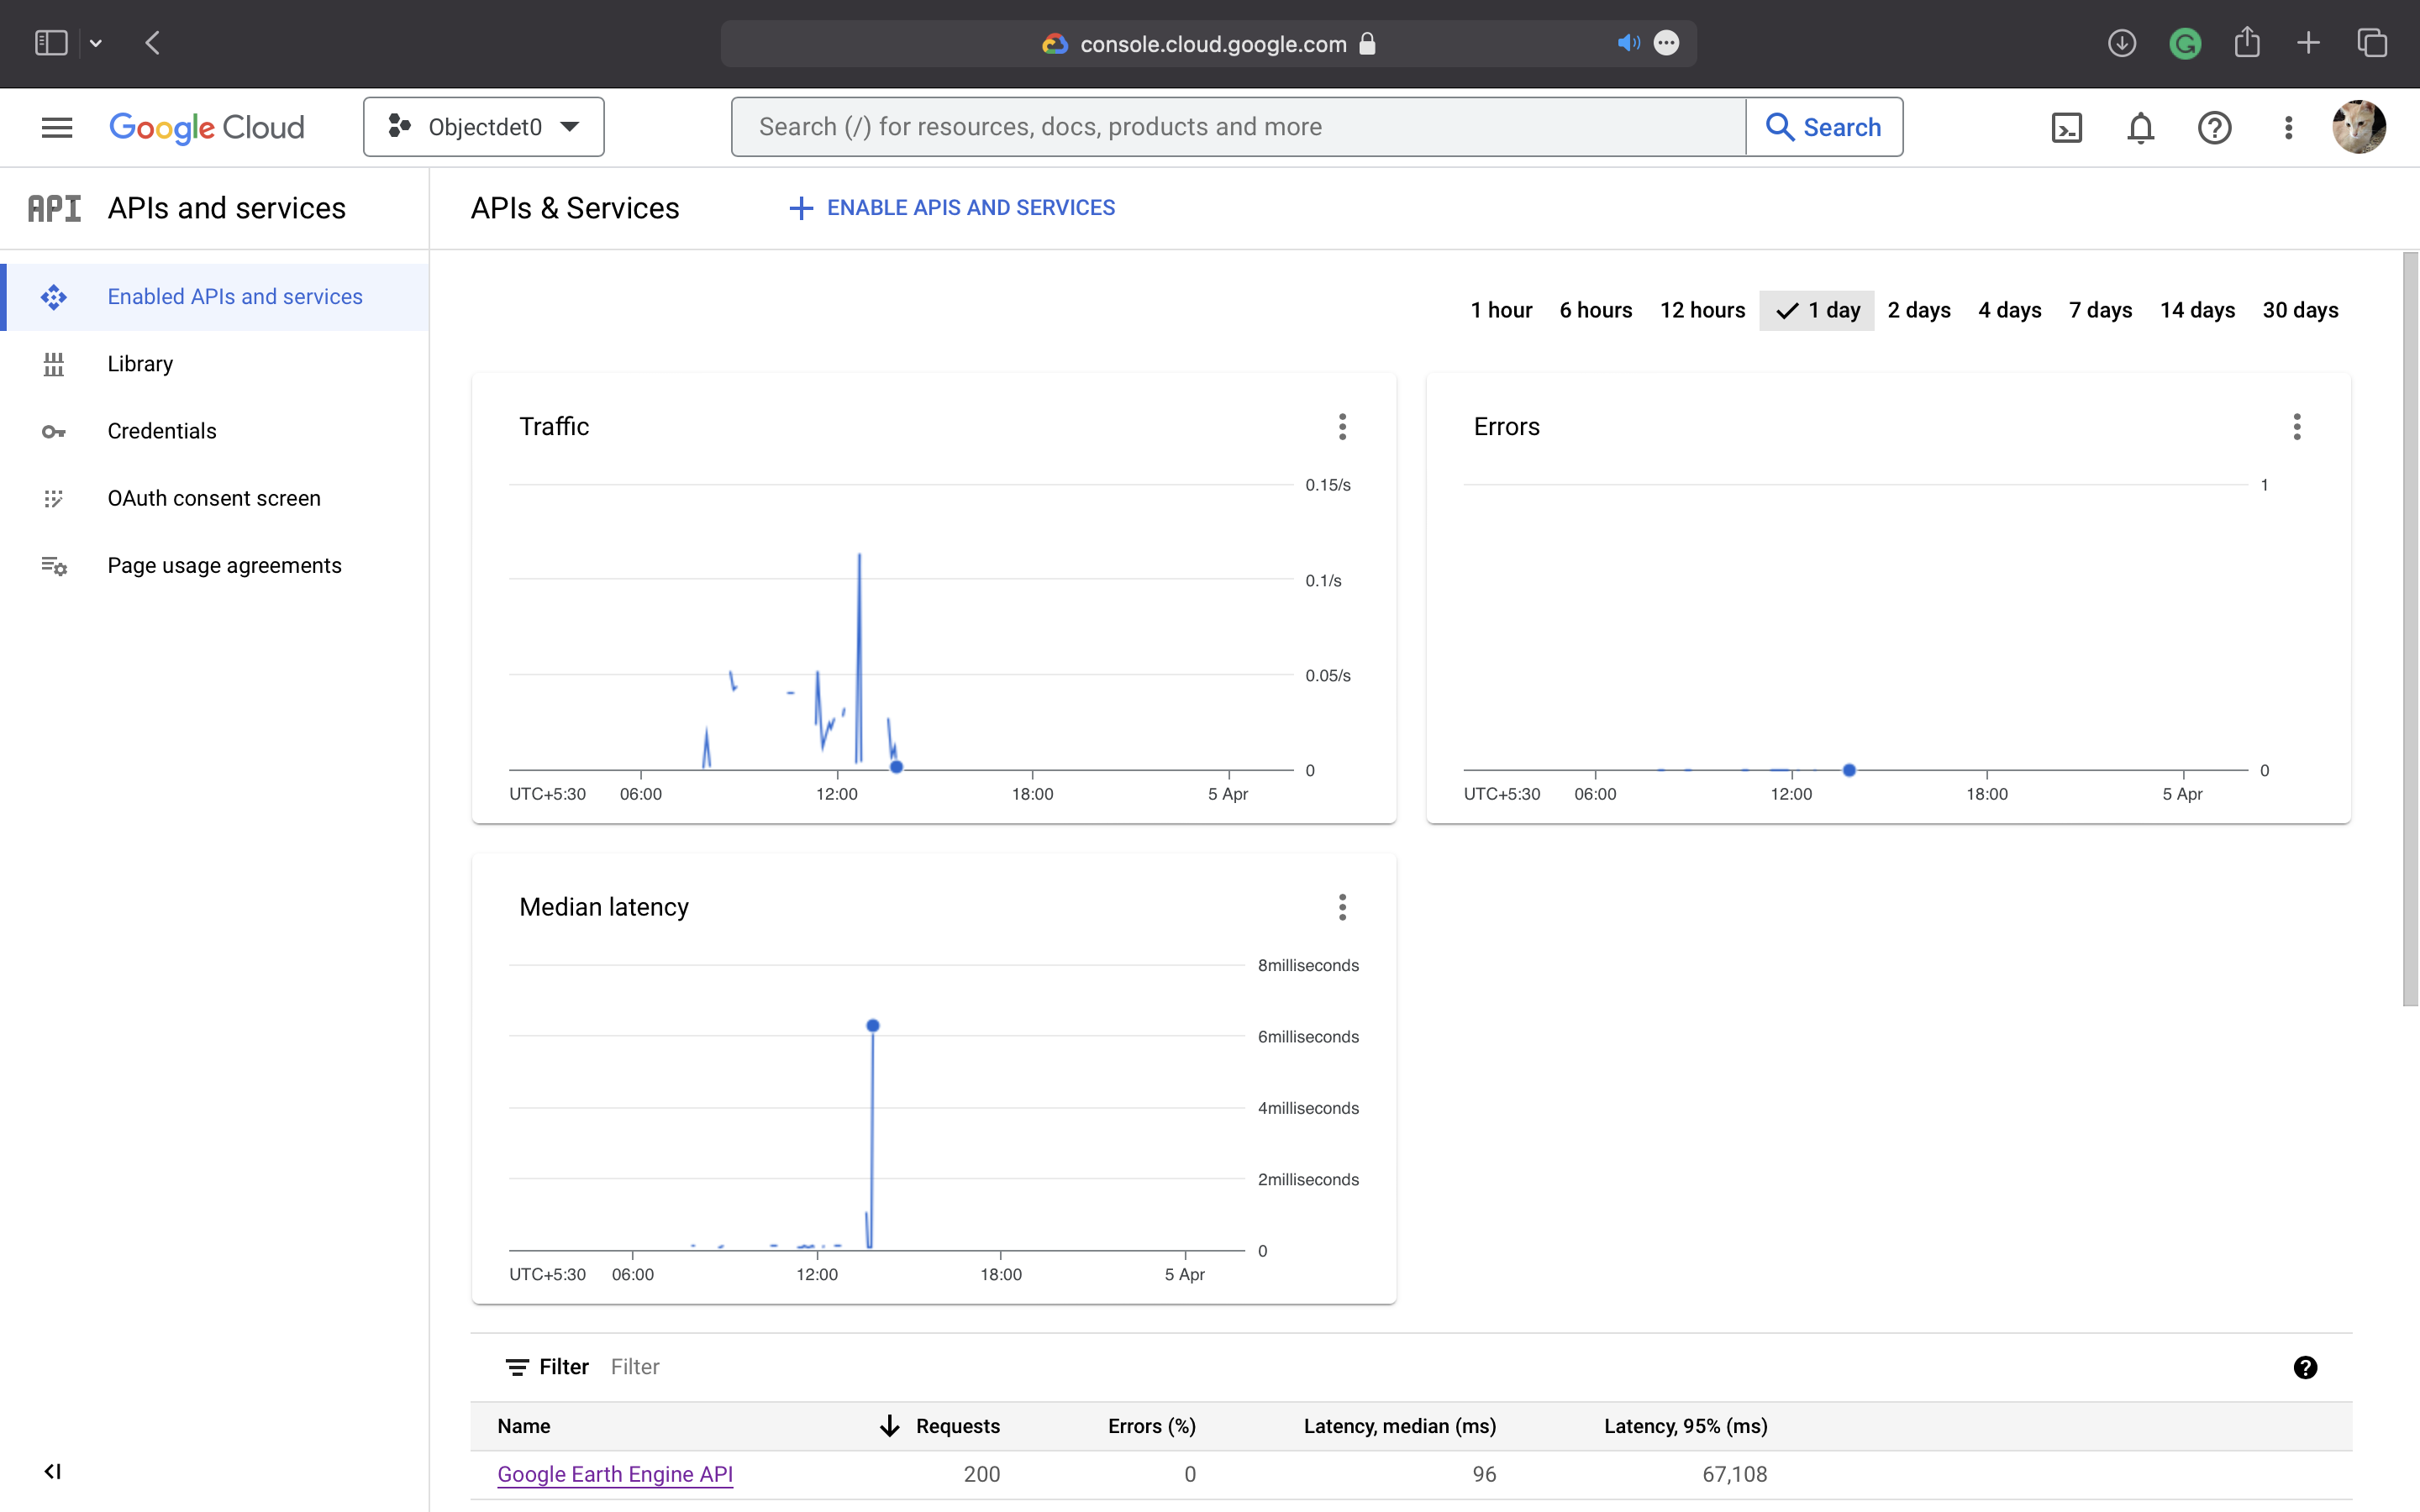
\includegraphics[scale=0.34]{screenshts/1.png}
\subsection{GCP Service Accounts}
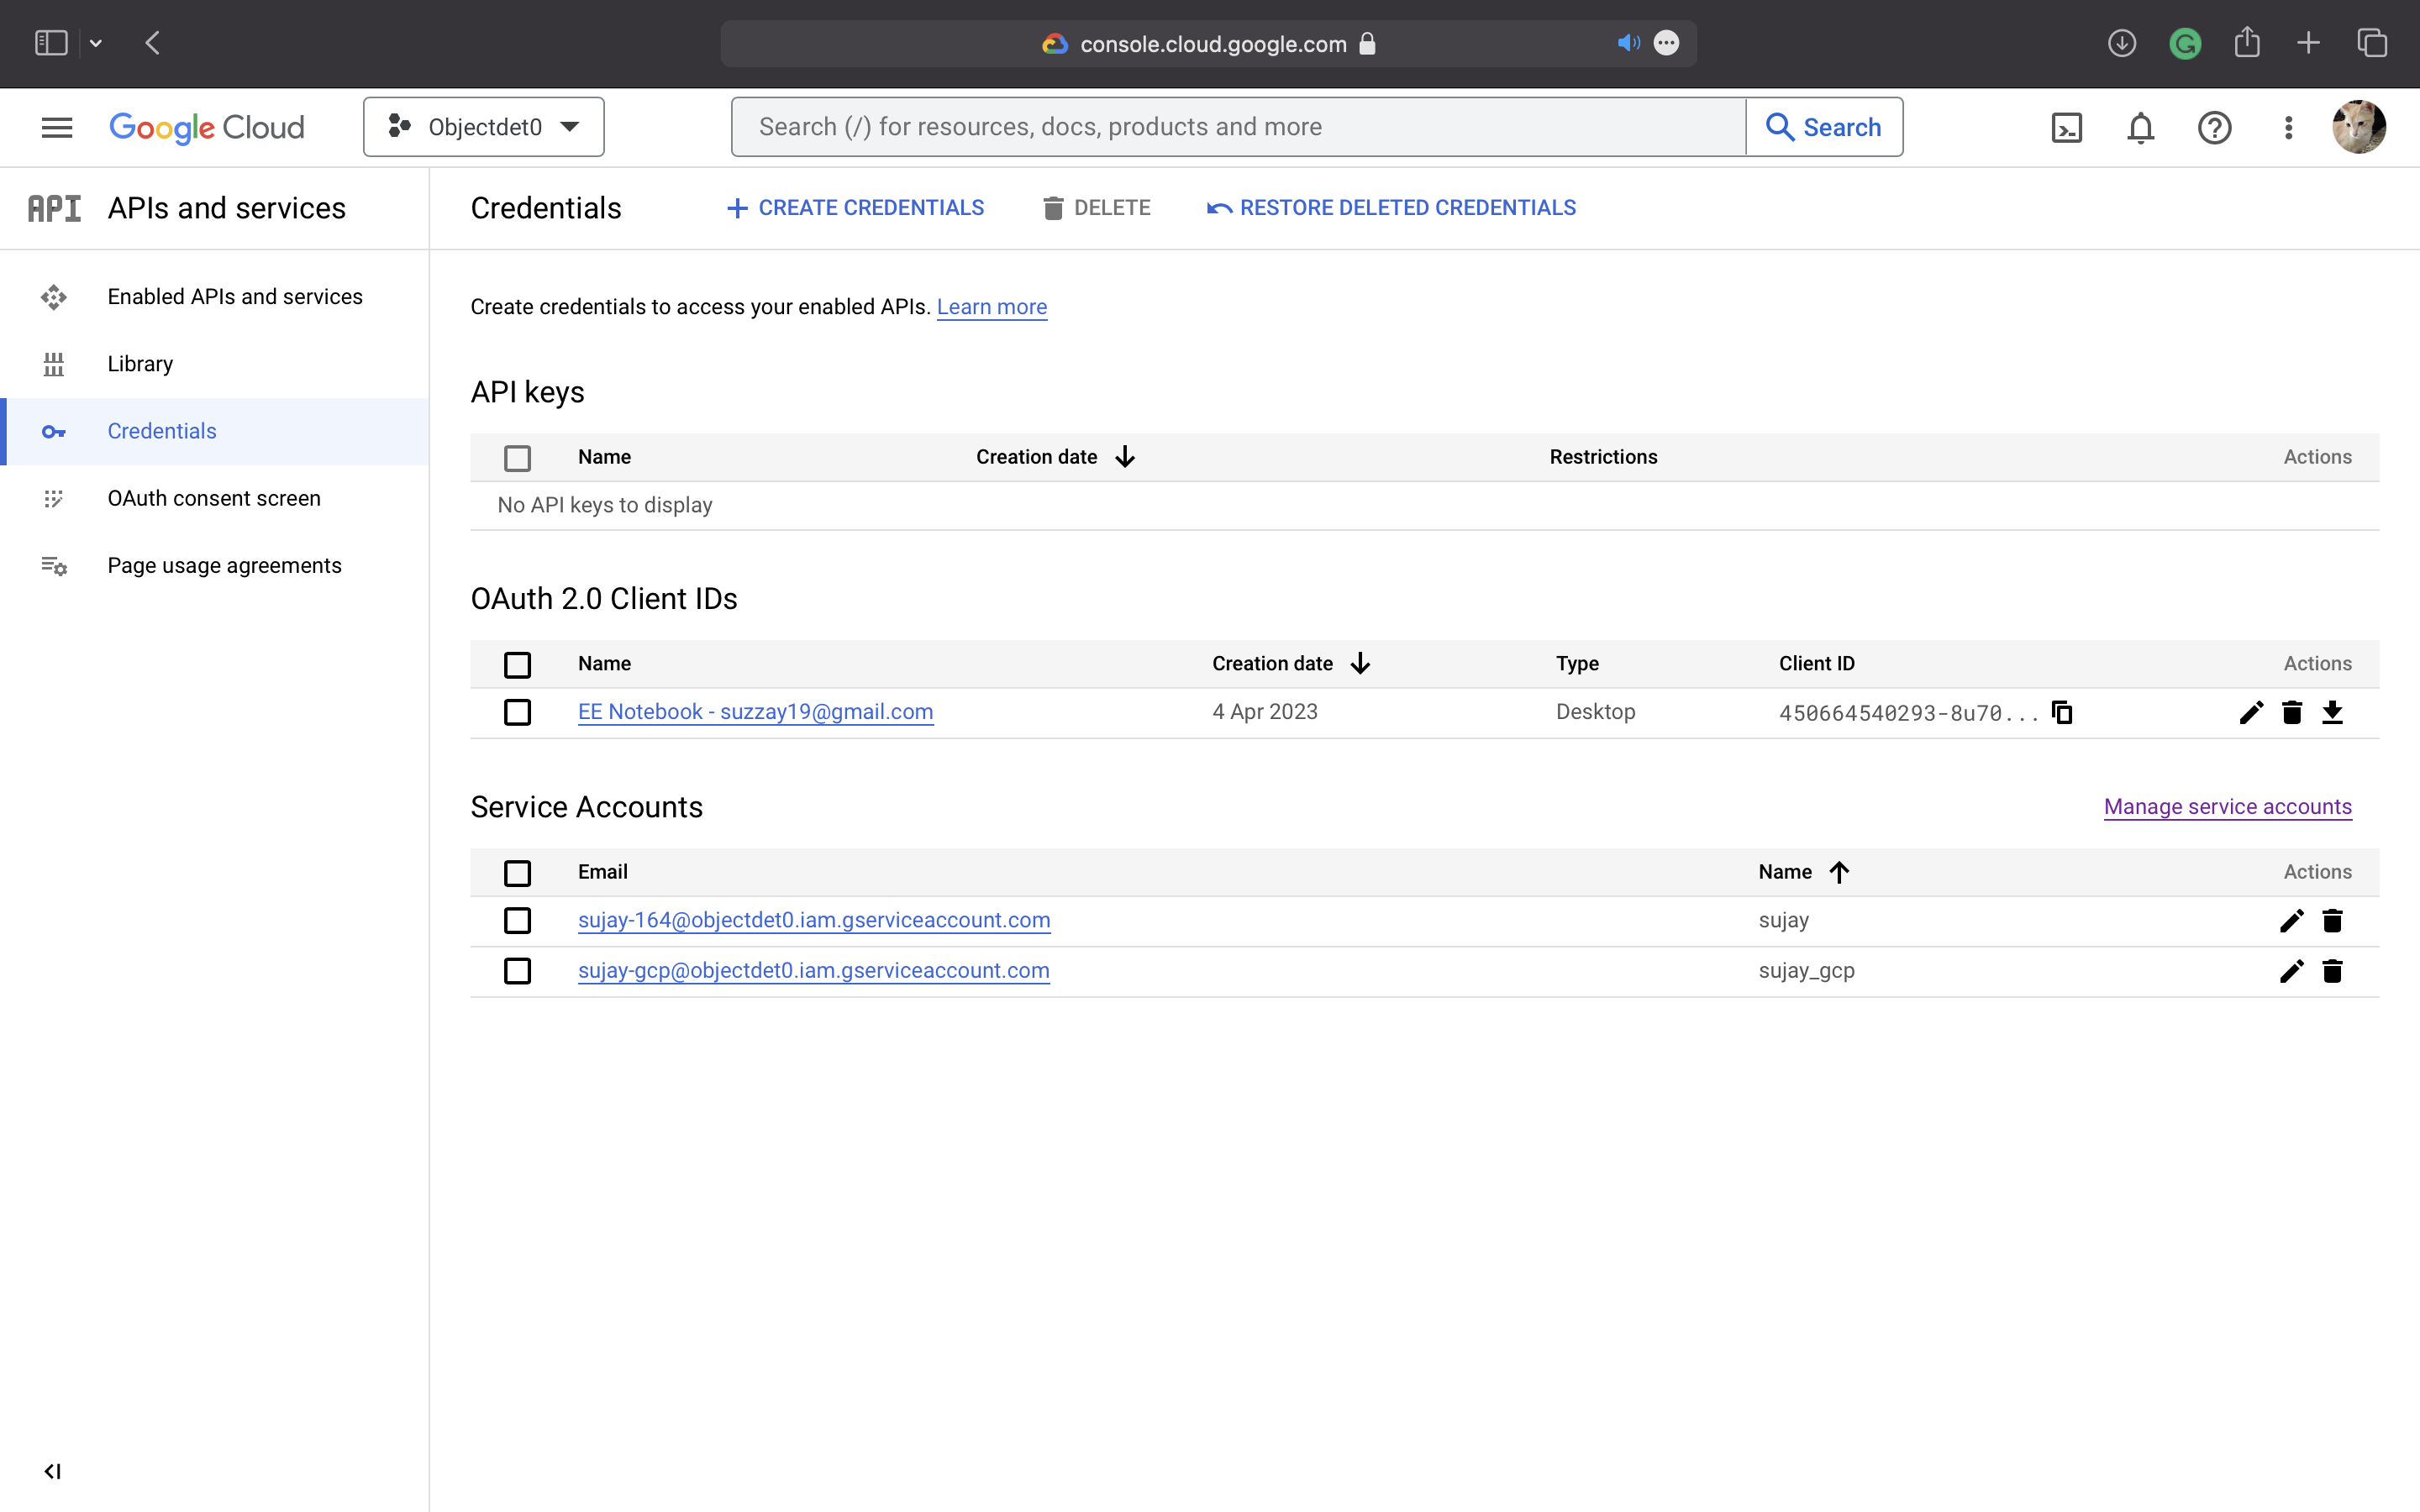
\includegraphics[scale=0.3]{screenshts/2.png}
\subsection{GCP Identity and Access Management}
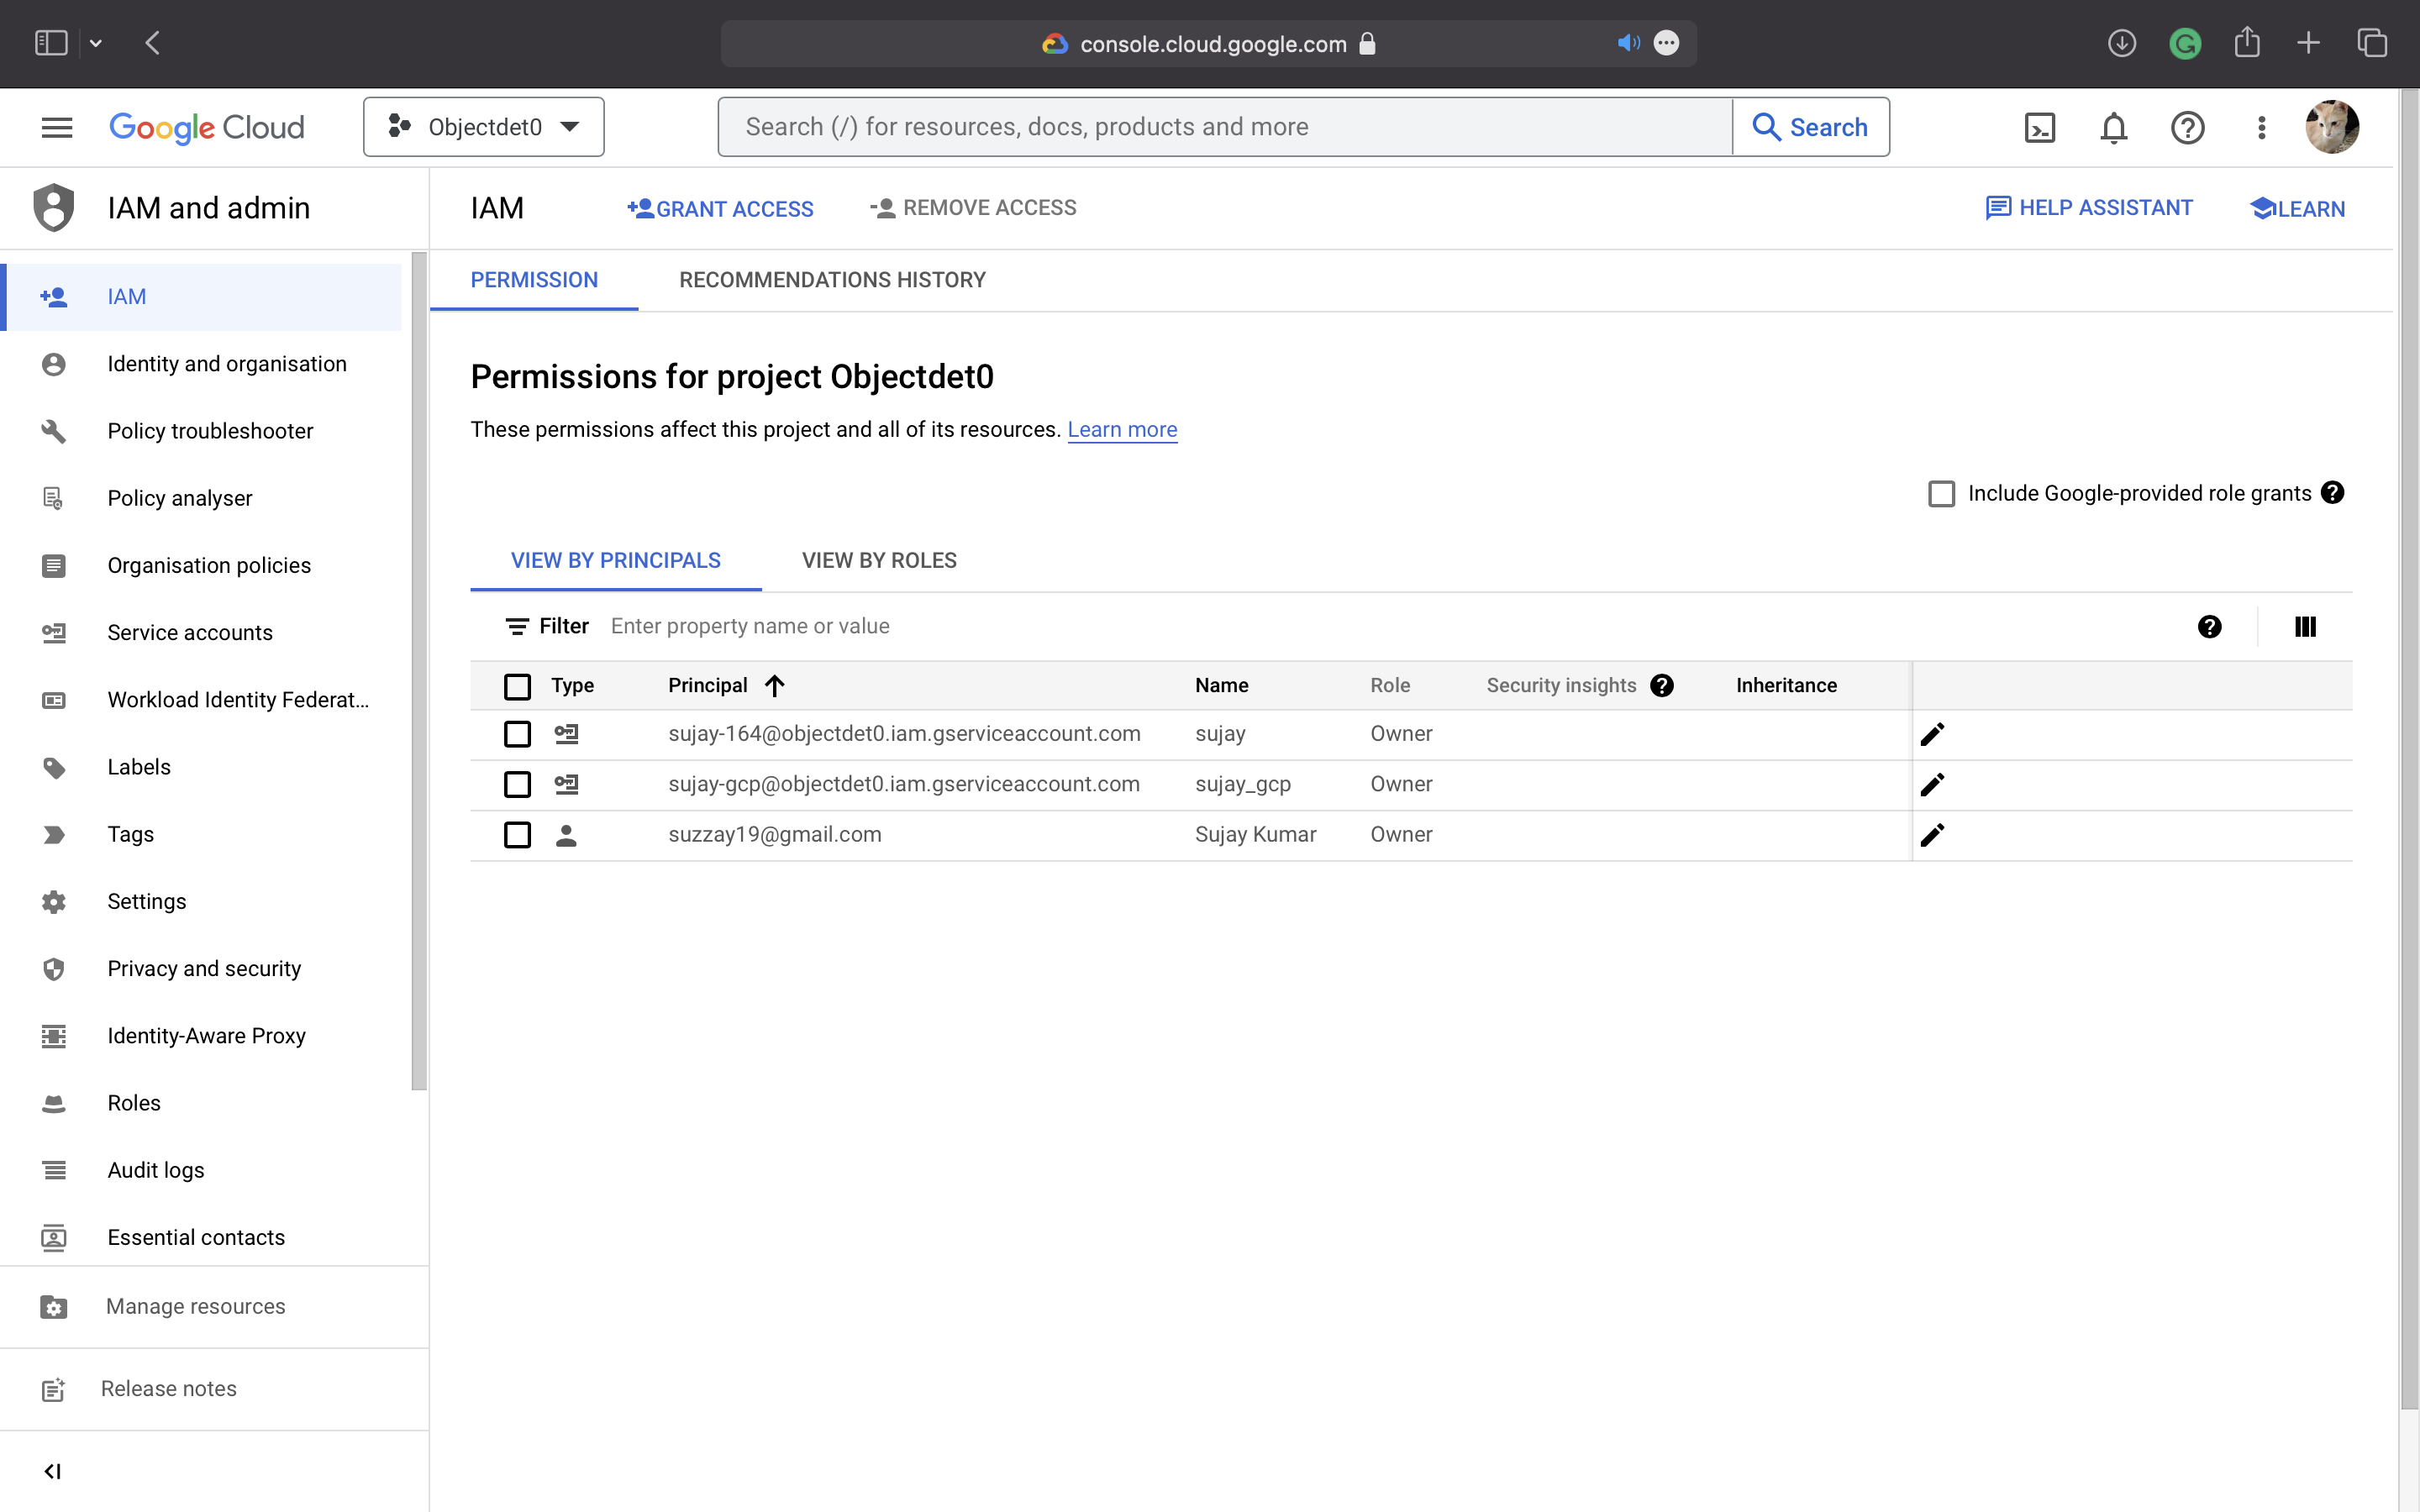
\includegraphics[scale=0.3]{screenshts/3.png}

\section{Data Analysis and Data Visualization}
\begin{lstlisting}[language=JavaScript]
// Determine 10-year mean LSTs

/**** Start of imports. If edited, may not auto-convert in the playground. ****/
var VisPar = {"opacity":1,"bands":["constant"],"min":-5,"max":40,"palette":["002bff","00ff36","fbff00","ff0000"]};
/***** End of imports. If edited, may not auto-convert in the playground. *****/
//variables
var numyears=10; //number of years
var firstyear=2005; //first year (beast after 2002)

//function oneyear mean
var oneyearmean=function(MYD,MOD){
var MYDm = MYD.mean();
var MODm = MOD.mean();
var LST_do=MODm.expression( //im transfering to celcius here so I don't have to worry about different band names
  '(0.02*LST - 273.15)',{
    'LST' : MODm.select('LST_Day_1km')
  });
var LST_no=MODm.expression(
  '(0.02*LST - 273.15)',{
    'LST' : MODm.select('LST_Night_1km')
  });
var LST_dy=MYDm.expression(
  '(0.02*LST - 273.15)',{
    'LST' : MYDm.select('LST_Day_1km')
  });
var LST_ny=MYDm.expression(
  '(0.02*LST - 273.15)',{
    'LST' : MYDm.select('LST_Night_1km')
  });
var LST = ee.ImageCollection([LST_dy,LST_ny,LST_do,LST_no]).mean();
//going with image collection to get the mean, couse than i don't have to fiure out how to work with the 'no value' pixels
  return LST;
};

//function 10 year mean month
var meanmonth=function(from,to,month){
var LST2=ee.List([]); //dummy to fill with LSTs

for (var year = firstyear; year < firstyear+numyears; year++) {
var quarter_from = ee.Date(year.toString() +from);
var quarter_to = ee.Date(year.toString() +to);
if (month == 12) {
  var yy=year+1;
    quarter_to = ee.Date(yy.toString() +to);
}
var MYD = ee.ImageCollection('MODIS/MYD11A1')
  .filterDate(quarter_from, quarter_to);
var MOD = ee.ImageCollection('MODIS/MOD11A1')
  .filterDate(quarter_from, quarter_to);
  LST=oneyearmean(MYD,MOD);
  LST2=LST2.add(LST);
}
var LST3=ee.ImageCollection(LST2);
return LST3.mean();
};

//start main code
var LST= ee.Image.constant(0); //dummy to fill with LSTs
for (var month=1;month<13;month++){
   var m =month+1;
  var daypermonth=31;
  if (month == 2){
    daypermonth=28;
  } else if  (month == 4 | month == 6 | month == 9 | month == 11) {
    daypermonth=30;
  }
  var from=('-'+month.toString()+'-01');
  var to=('-'+m.toString()+'-01'); 
  if (month == 12) {
    var to=('-01-01');
} 
    LST=LST.add(meanmonth(from,to,month).multiply(ee.Image.constant(daypermonth)));
}
//print('LST',LST);
LST=LST.expression(
  '(LST/365)',{
    'LST' : LST
  }); 
Map.setCenter(0, 0, 1); 
Map.addLayer(LST,VisPar,'LST');
 Export.image(LST, 'LST', {
  scale: 1000,
  maxPixels: 1e10
}); 
\end{lstlisting}
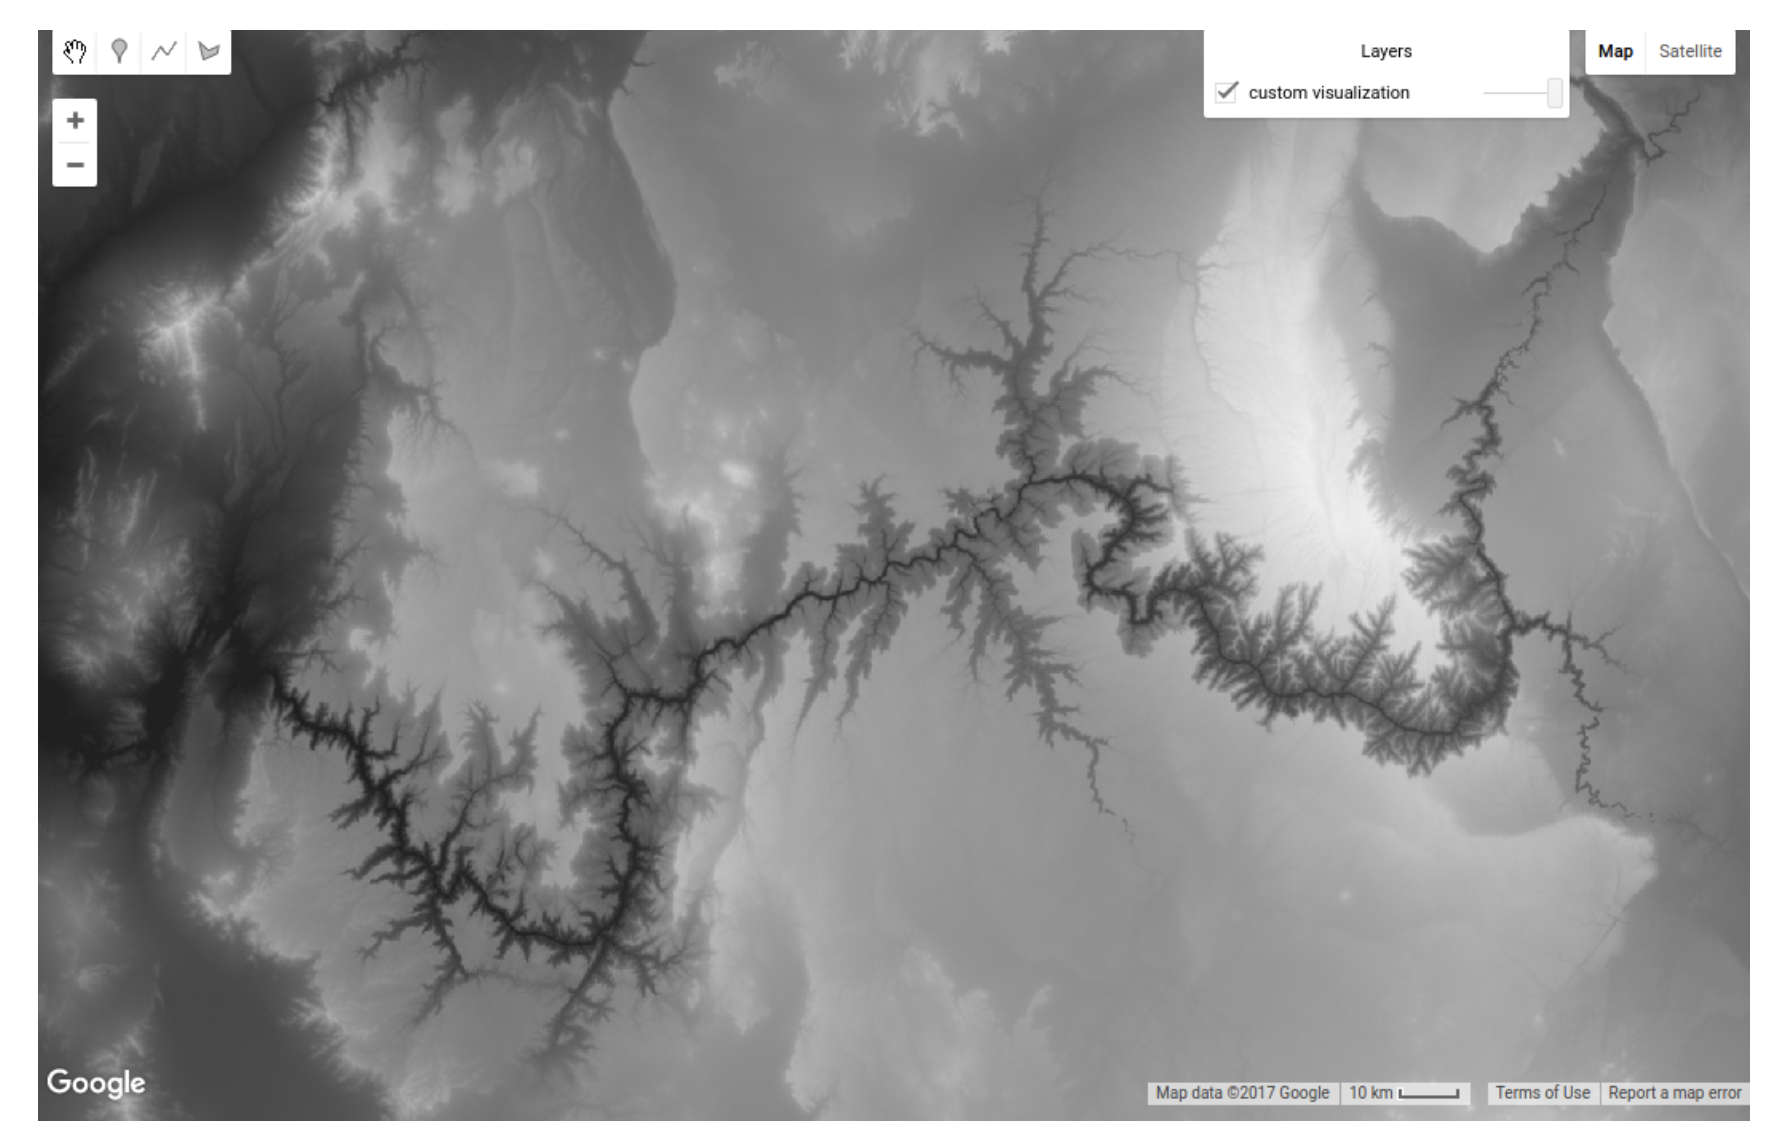
\includegraphics[scale=0.6]{screenshts/4.png}

\section{Pre-Procesing Using Patchify}
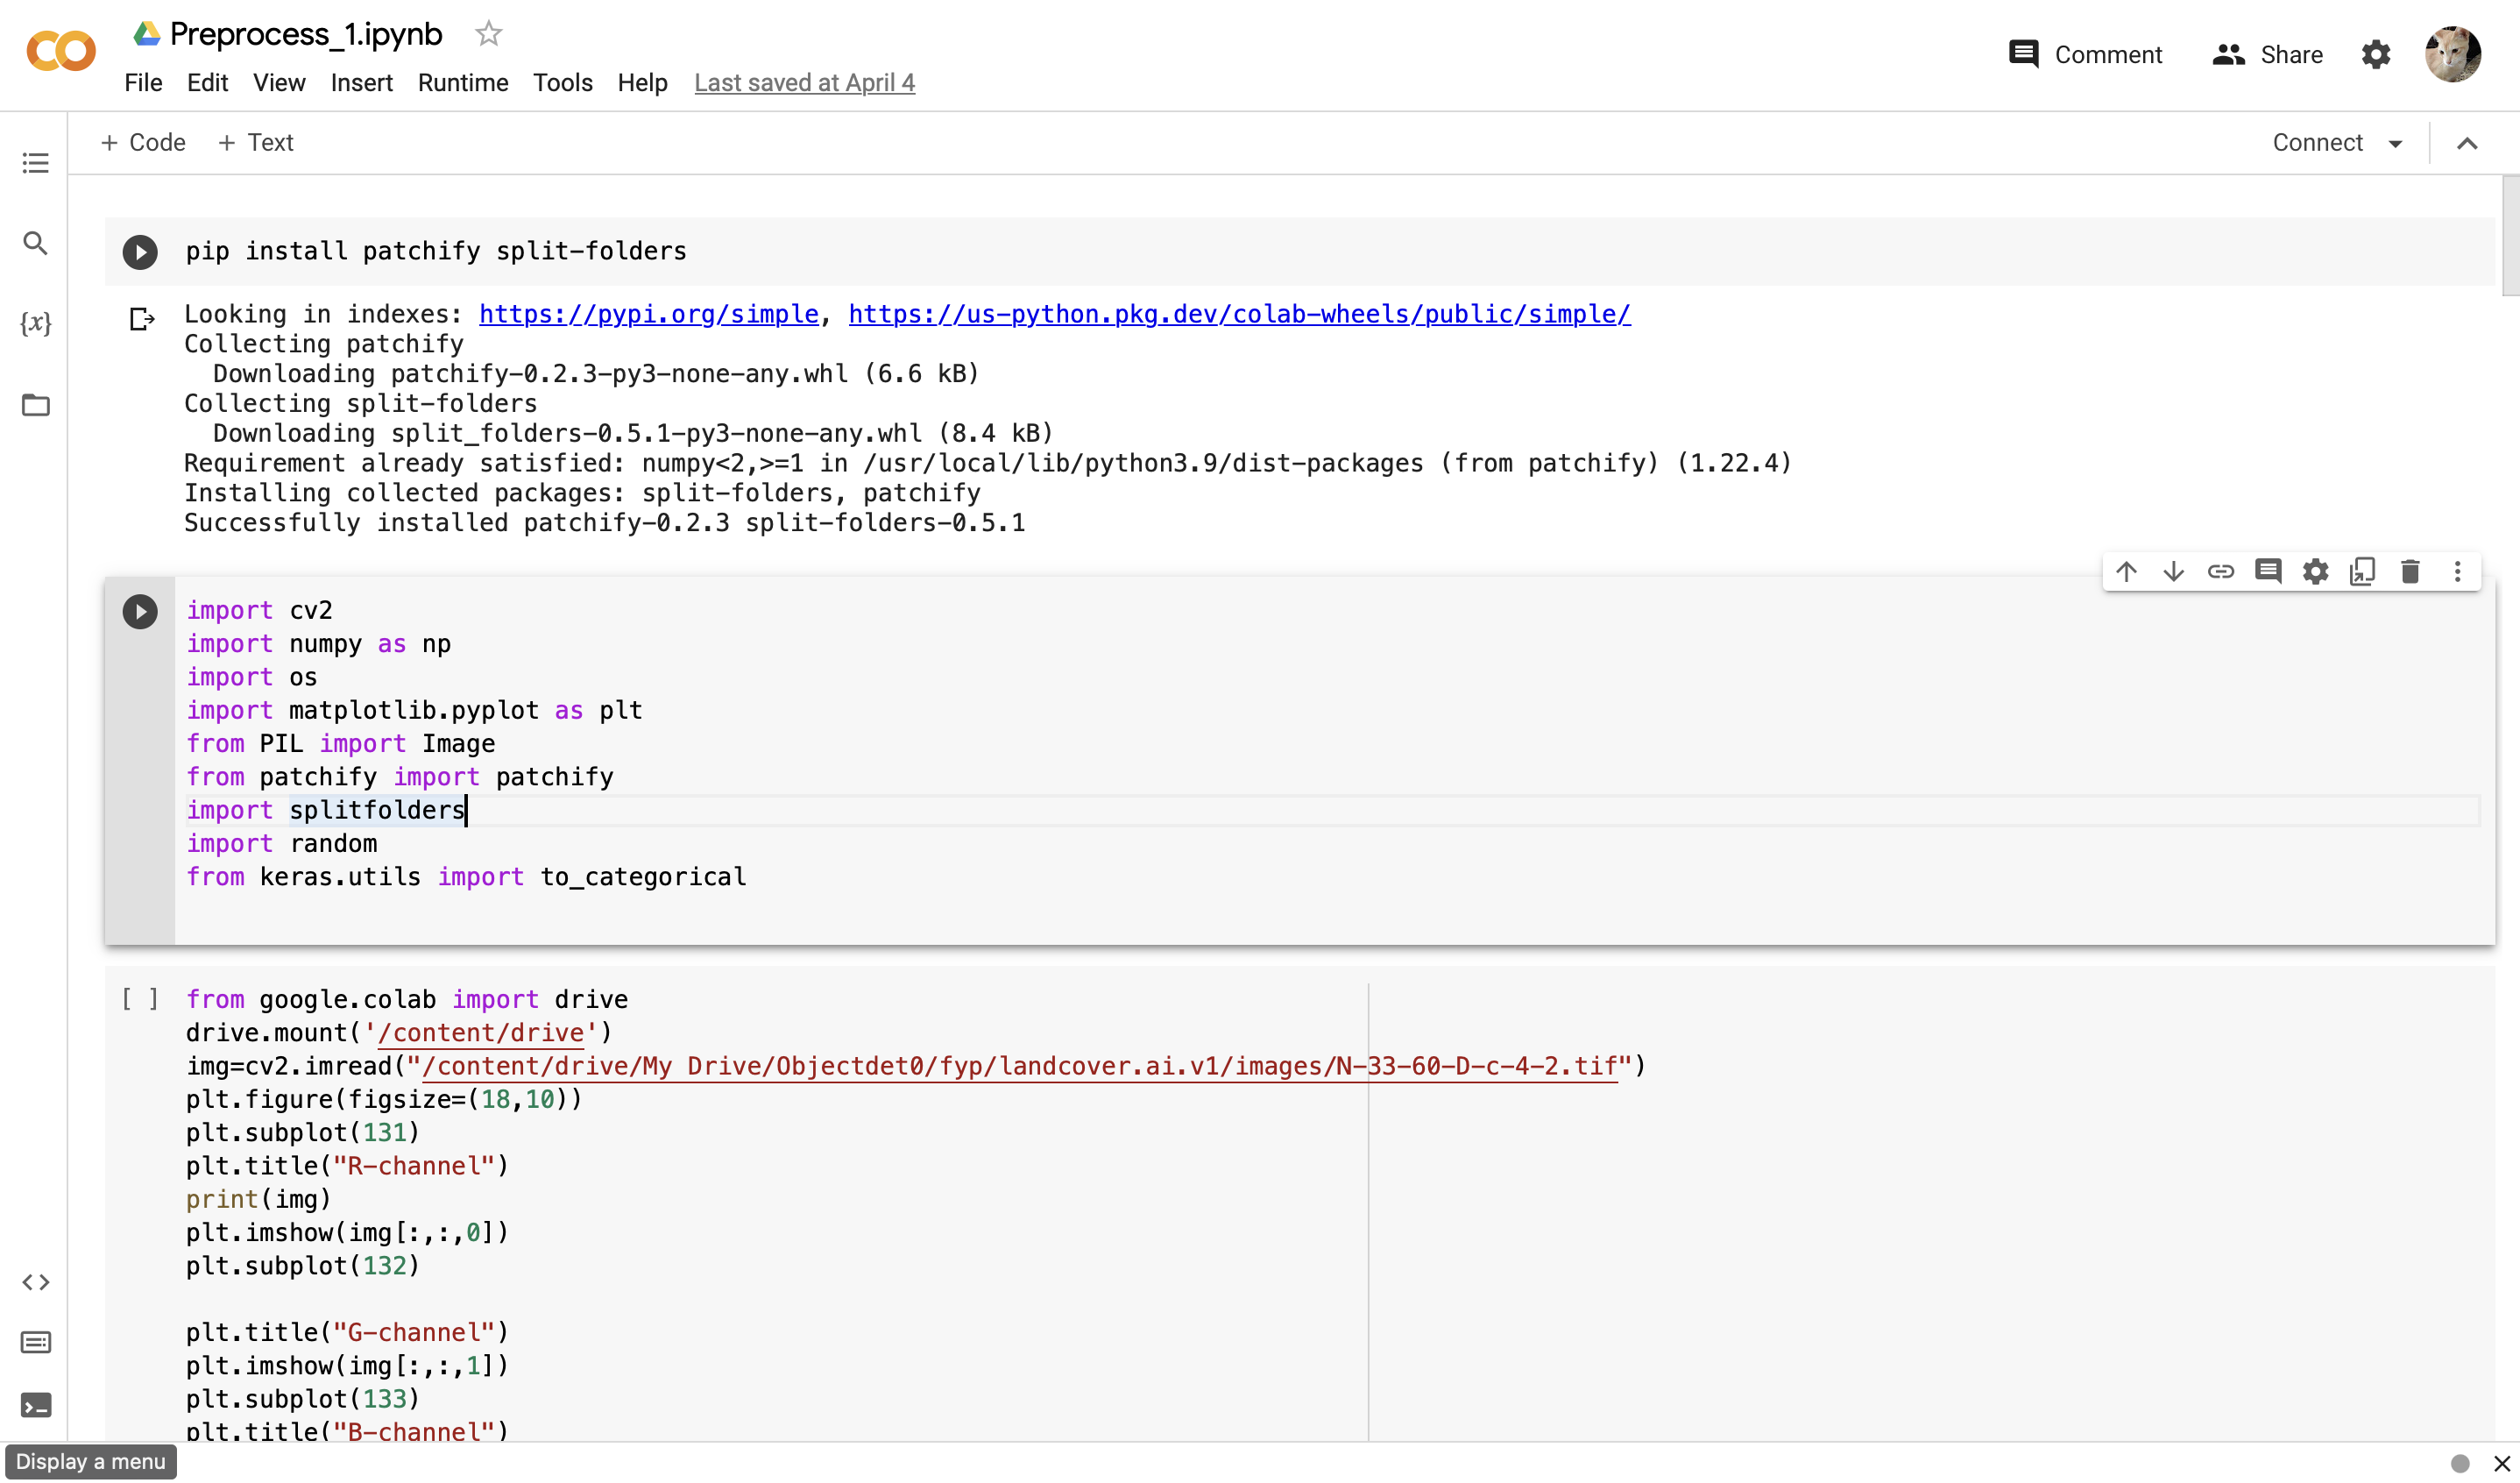
\includegraphics[scale=0.4]{screenshts/5.png}
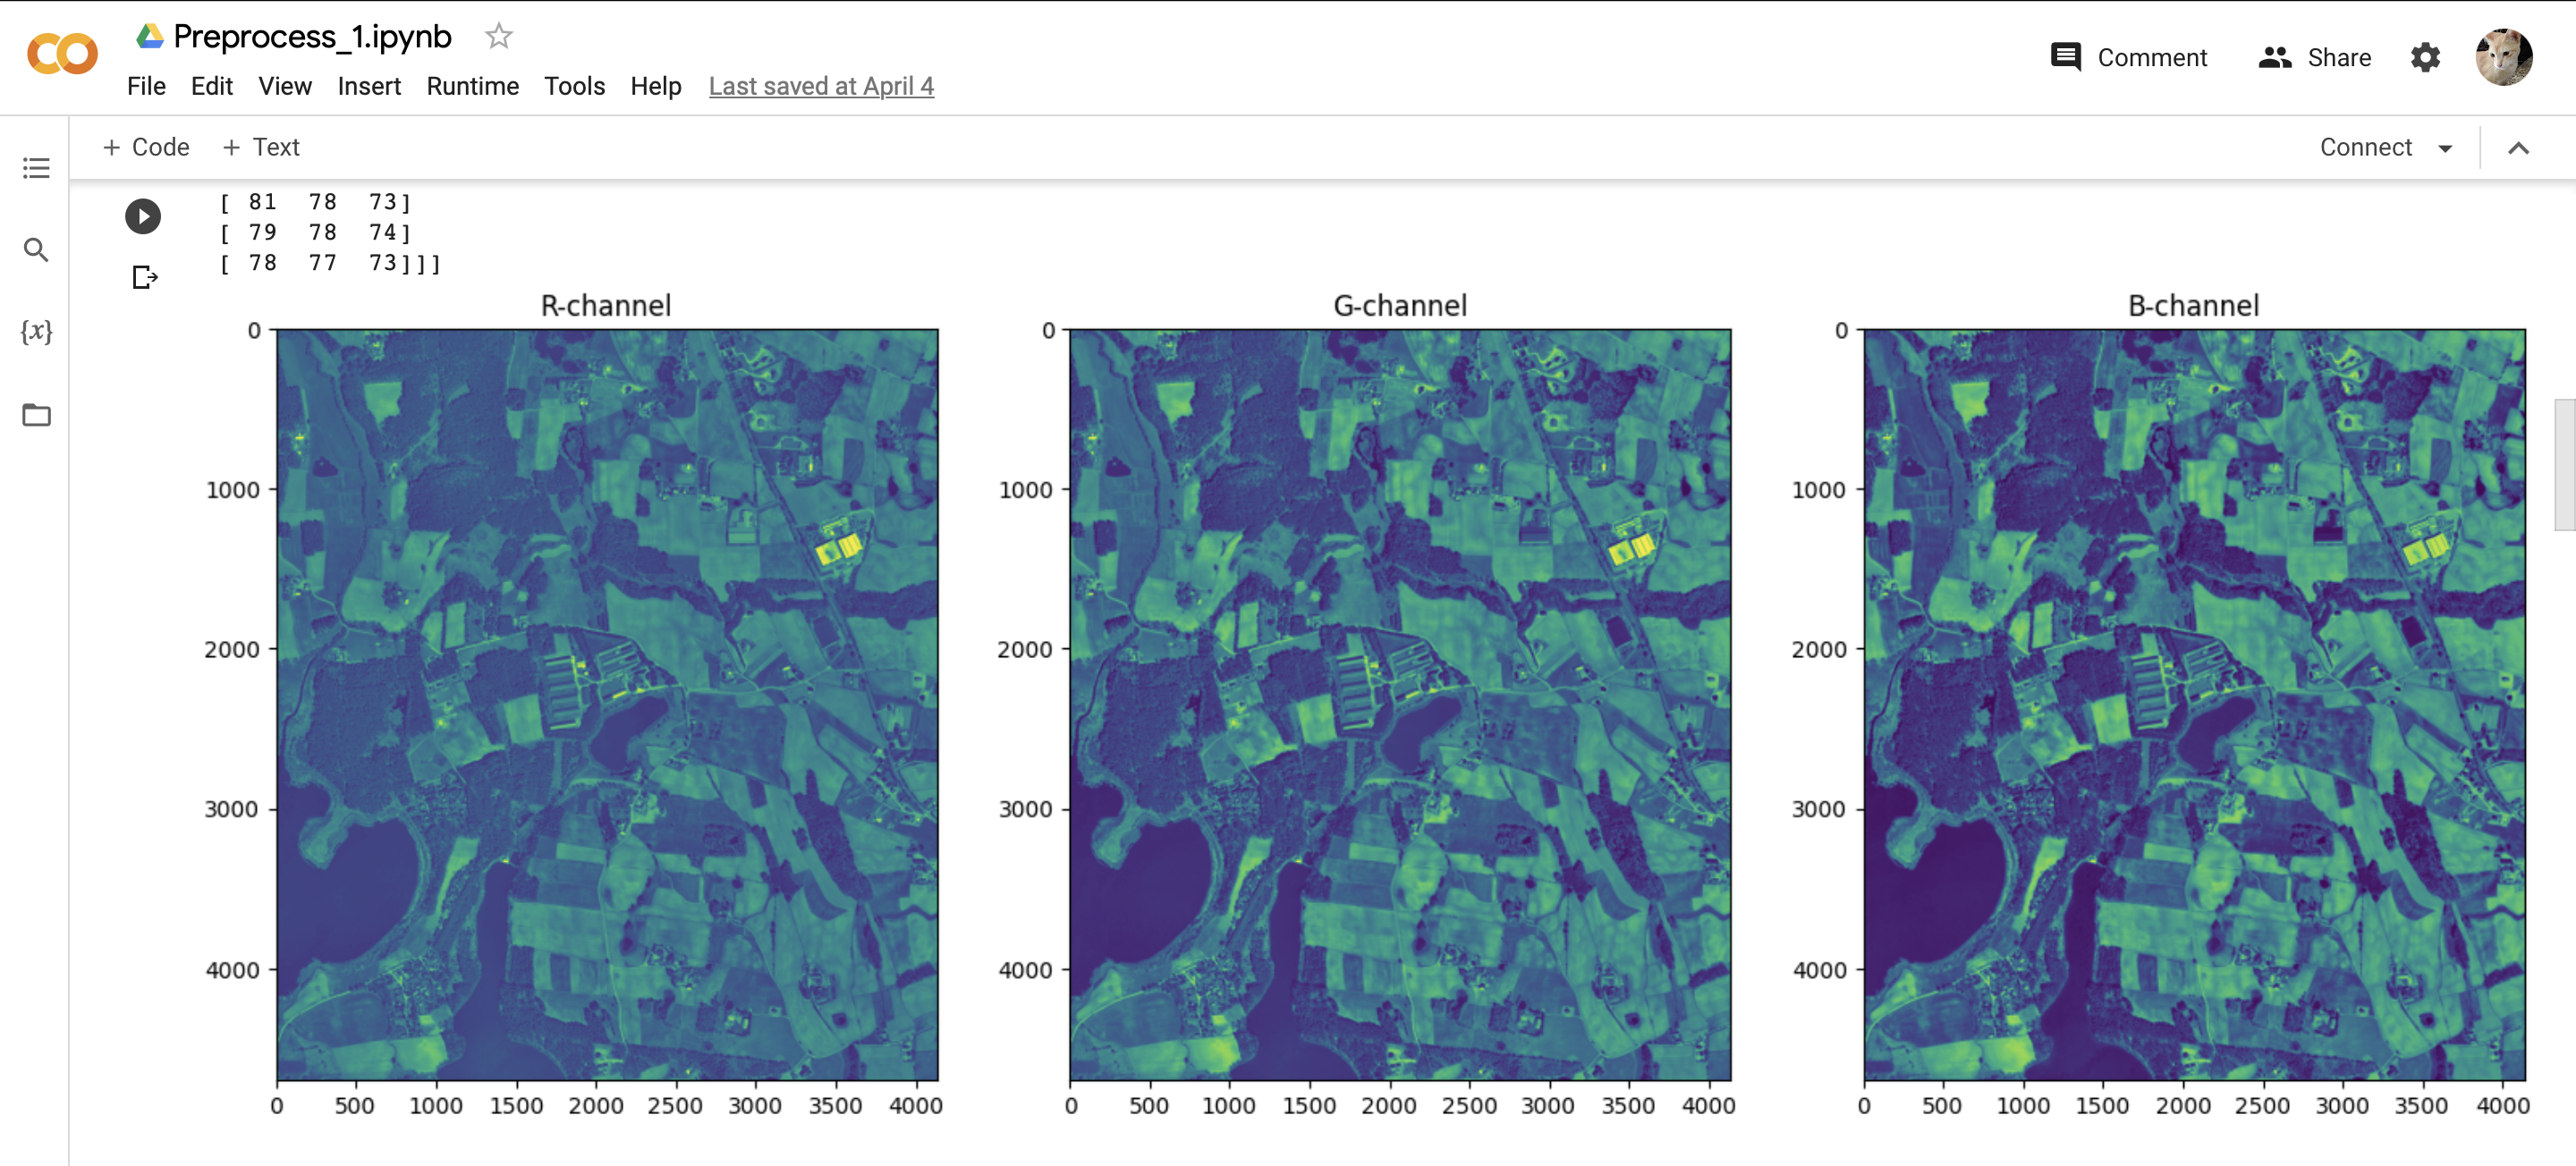
\includegraphics[scale=0.4]{screenshts/6.png}
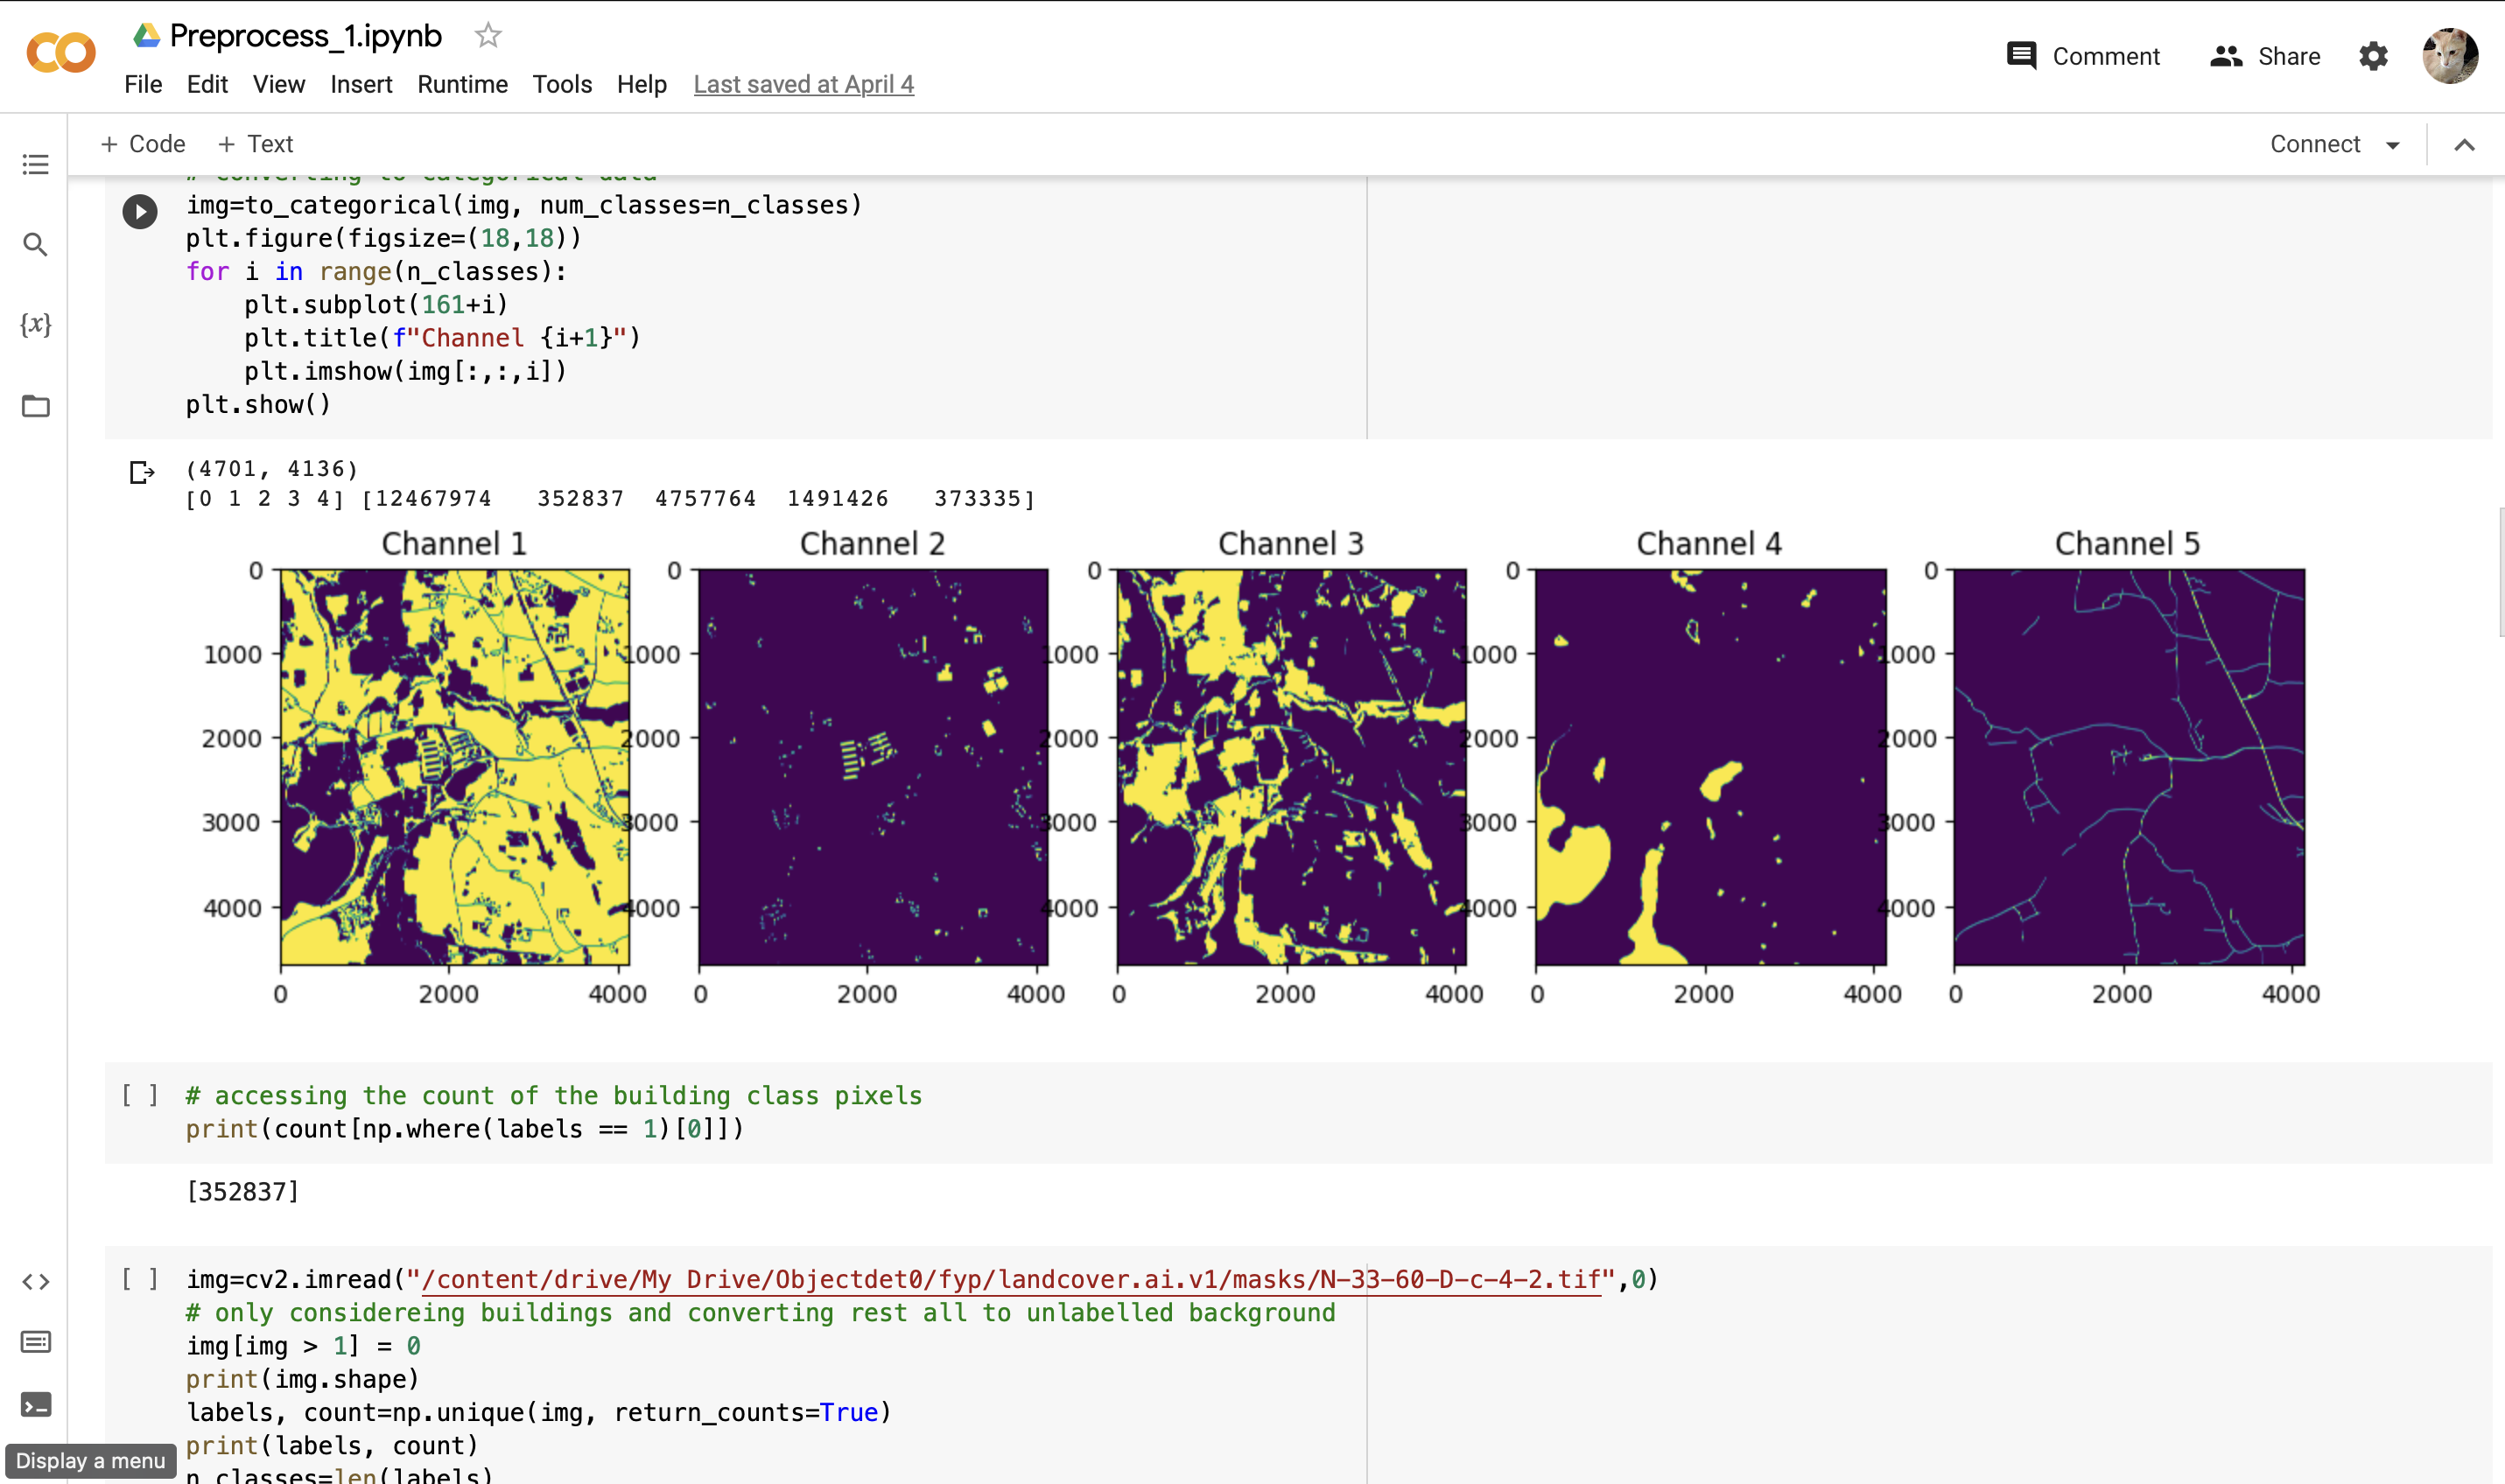
\includegraphics[scale=0.34]{screenshts/7.png}
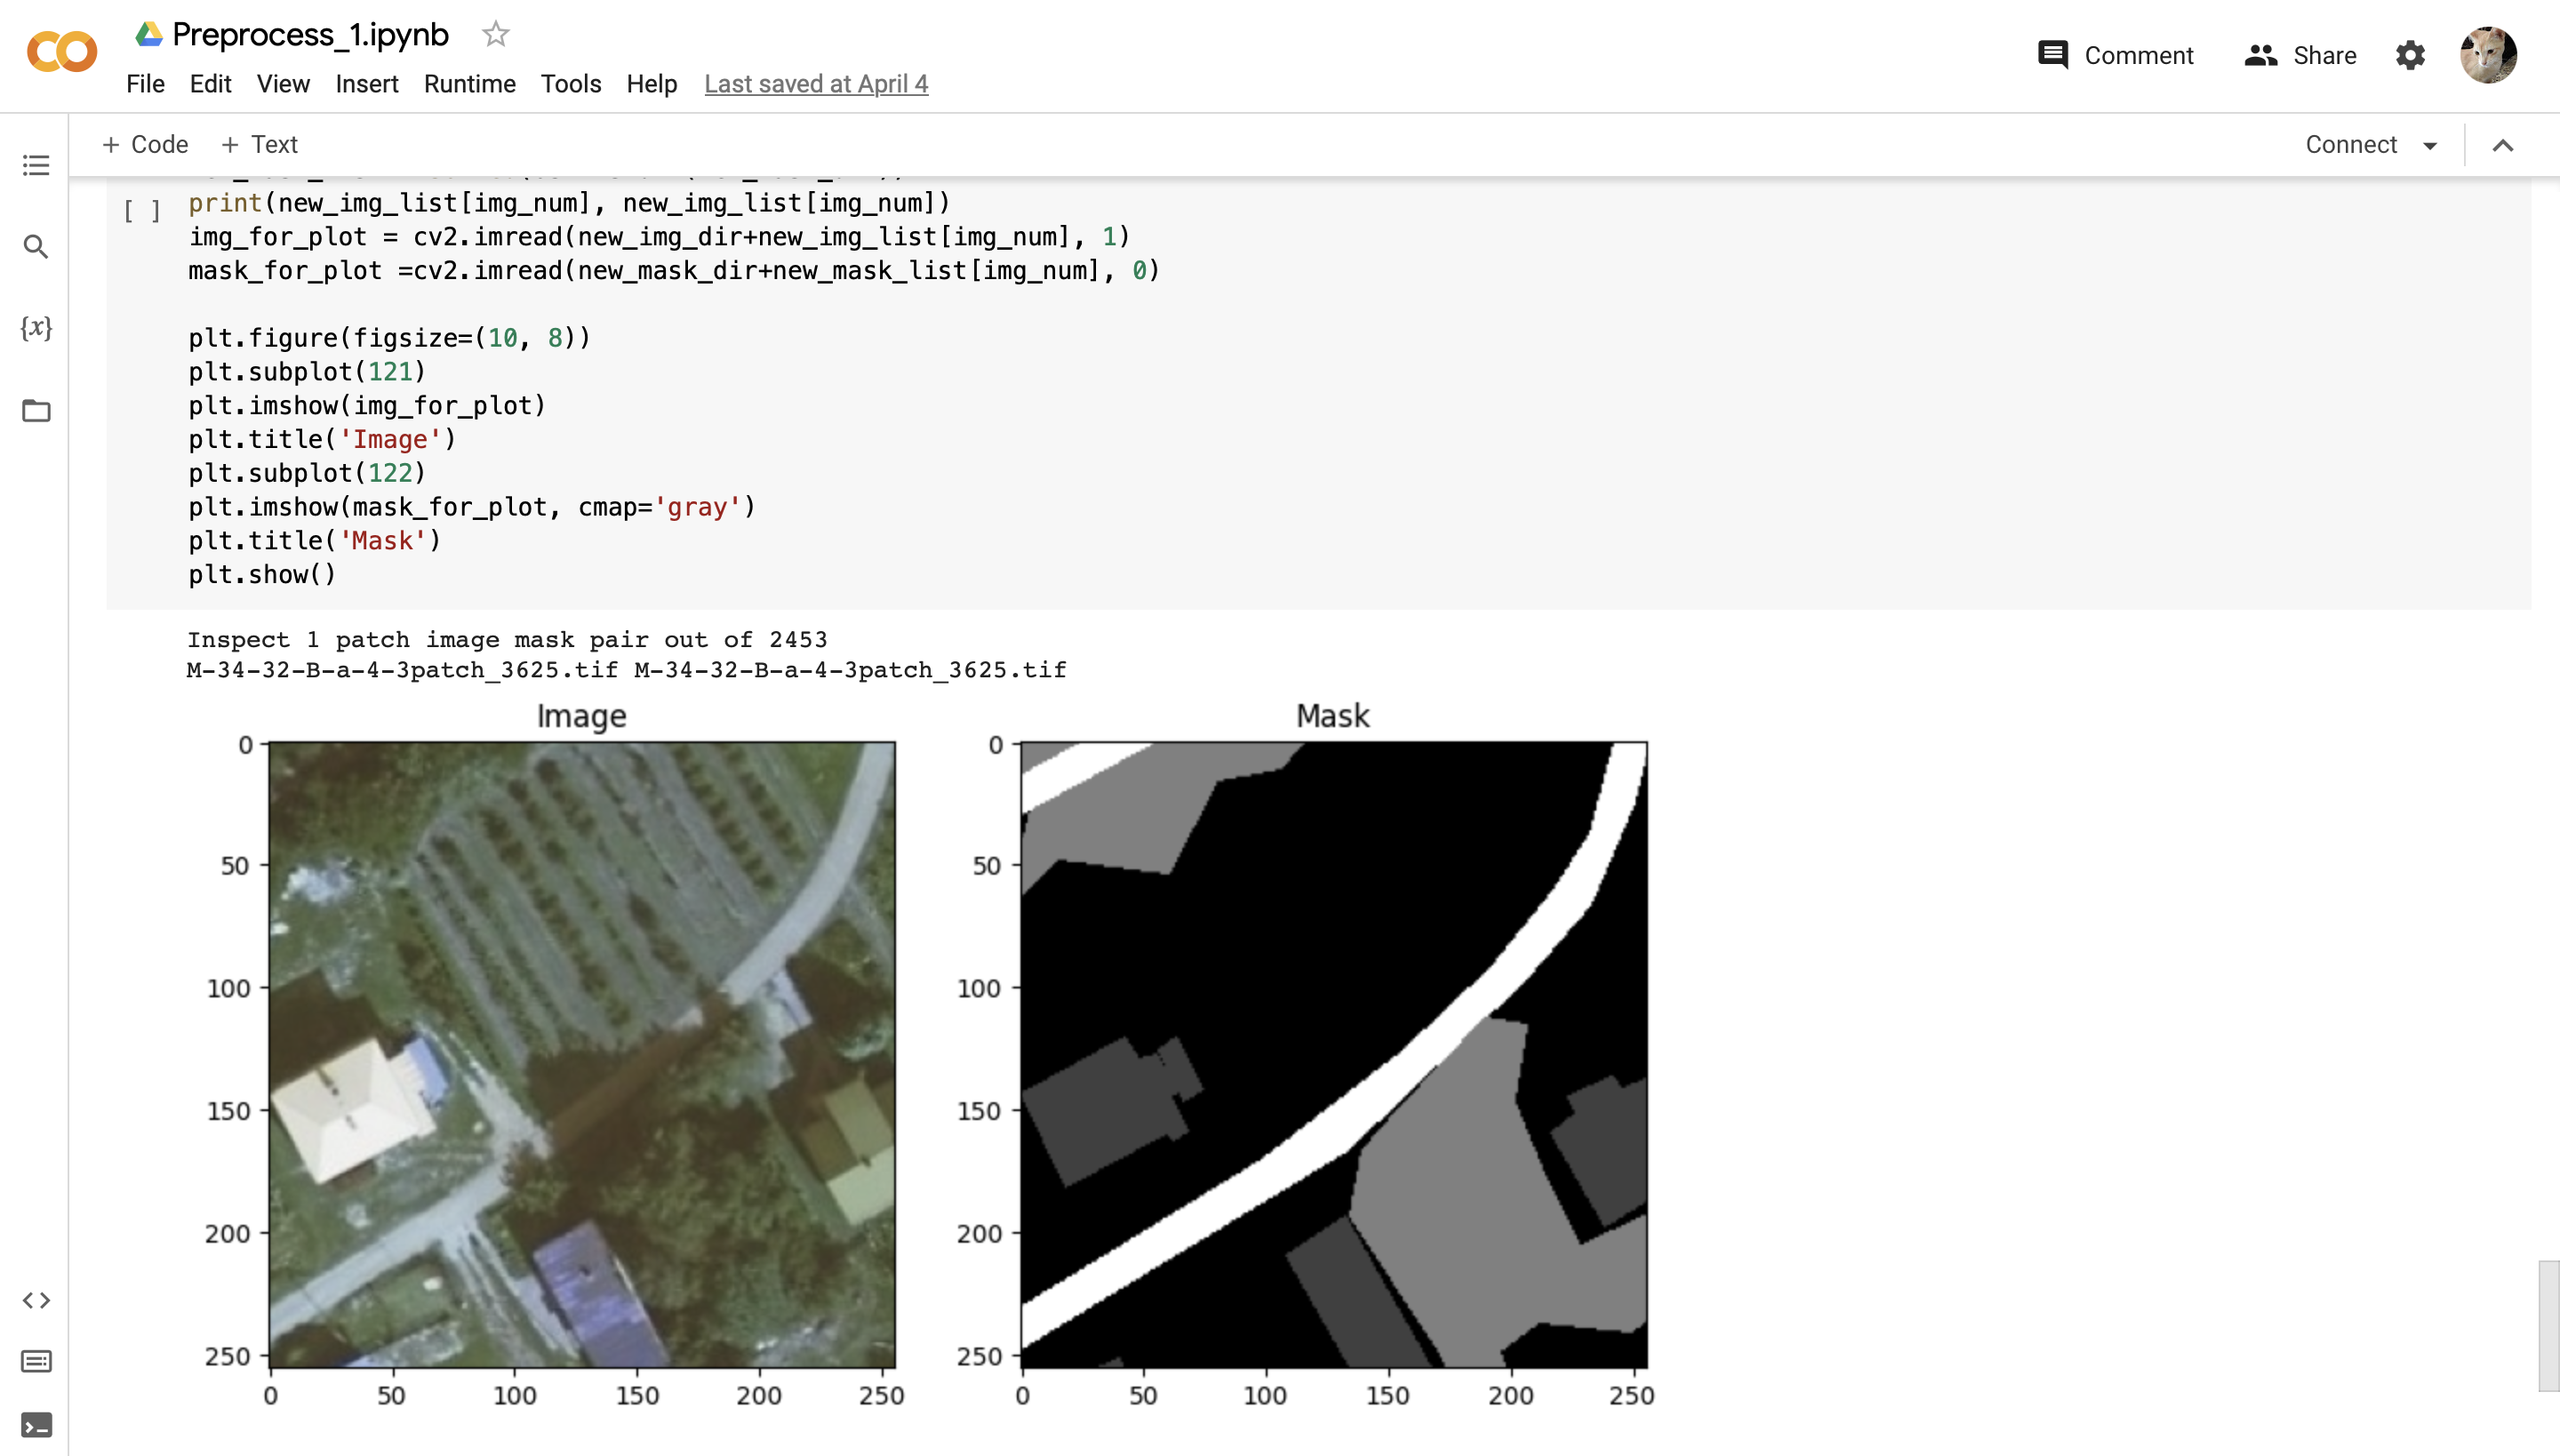
\includegraphics[scale=0.34]{screenshts/9.png}
\section{Training using UNet Architecture}
% 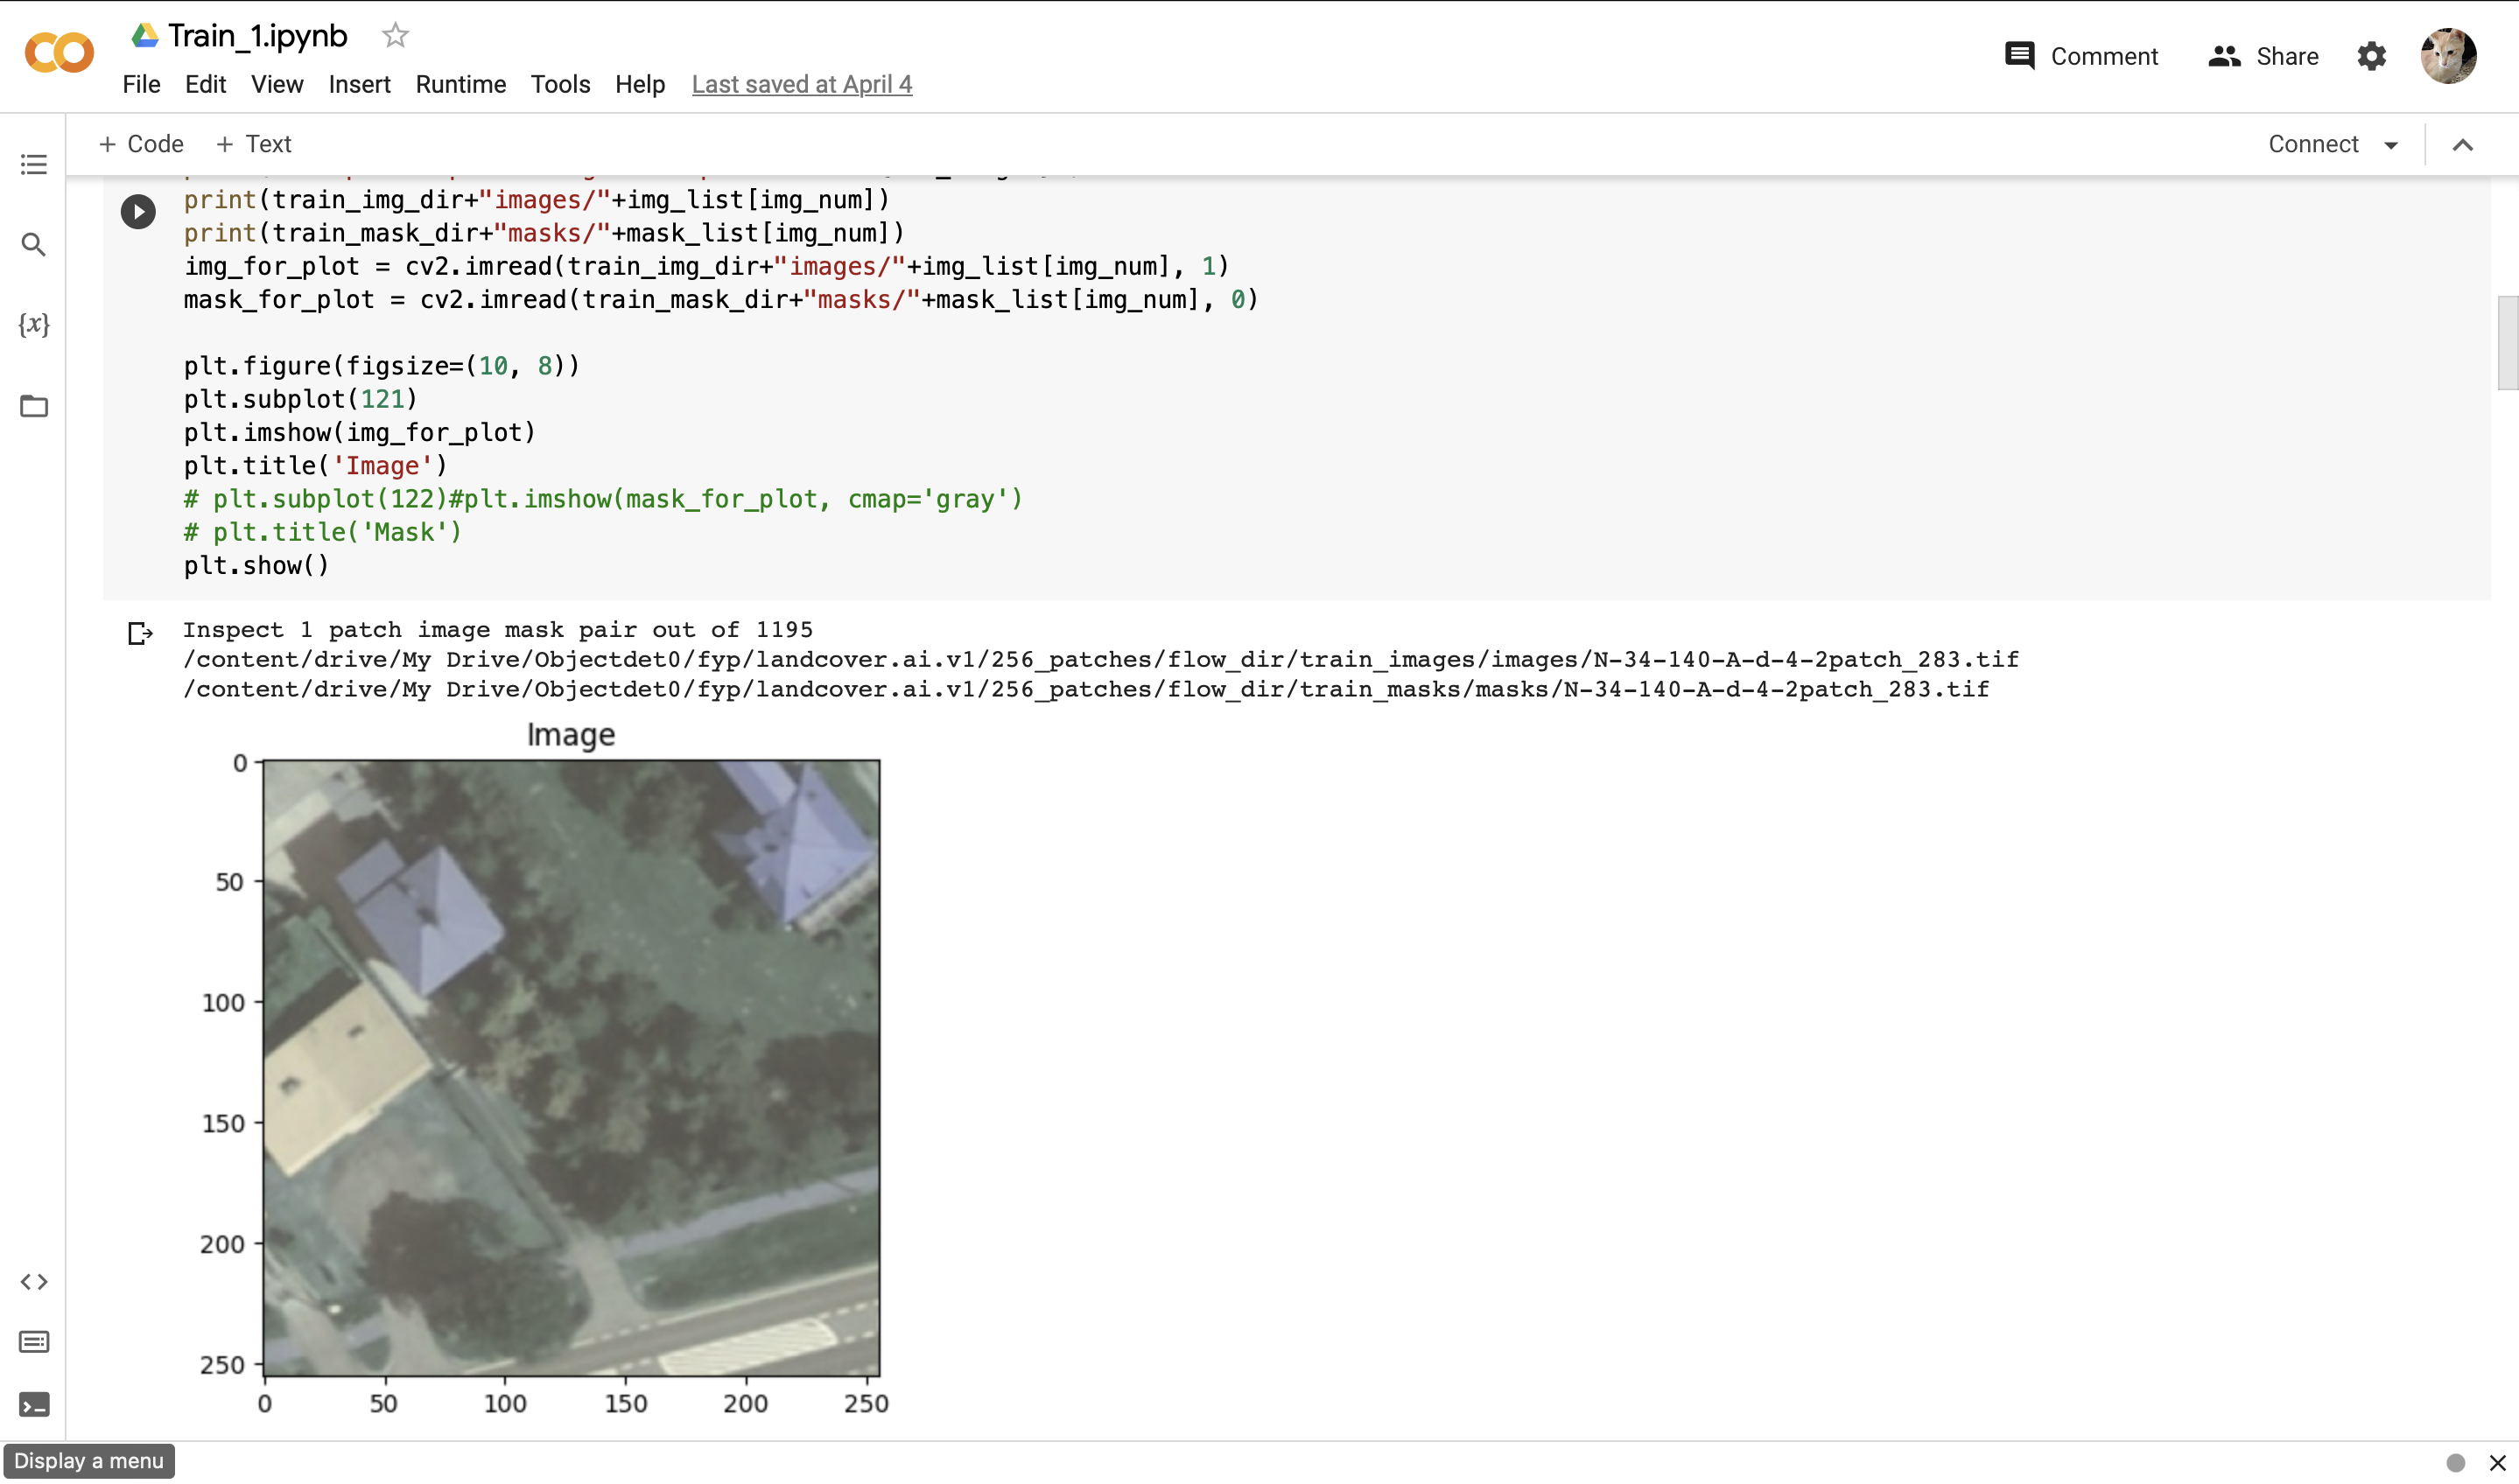
\includegraphics[scale=0.4]{screenshts/10.png}
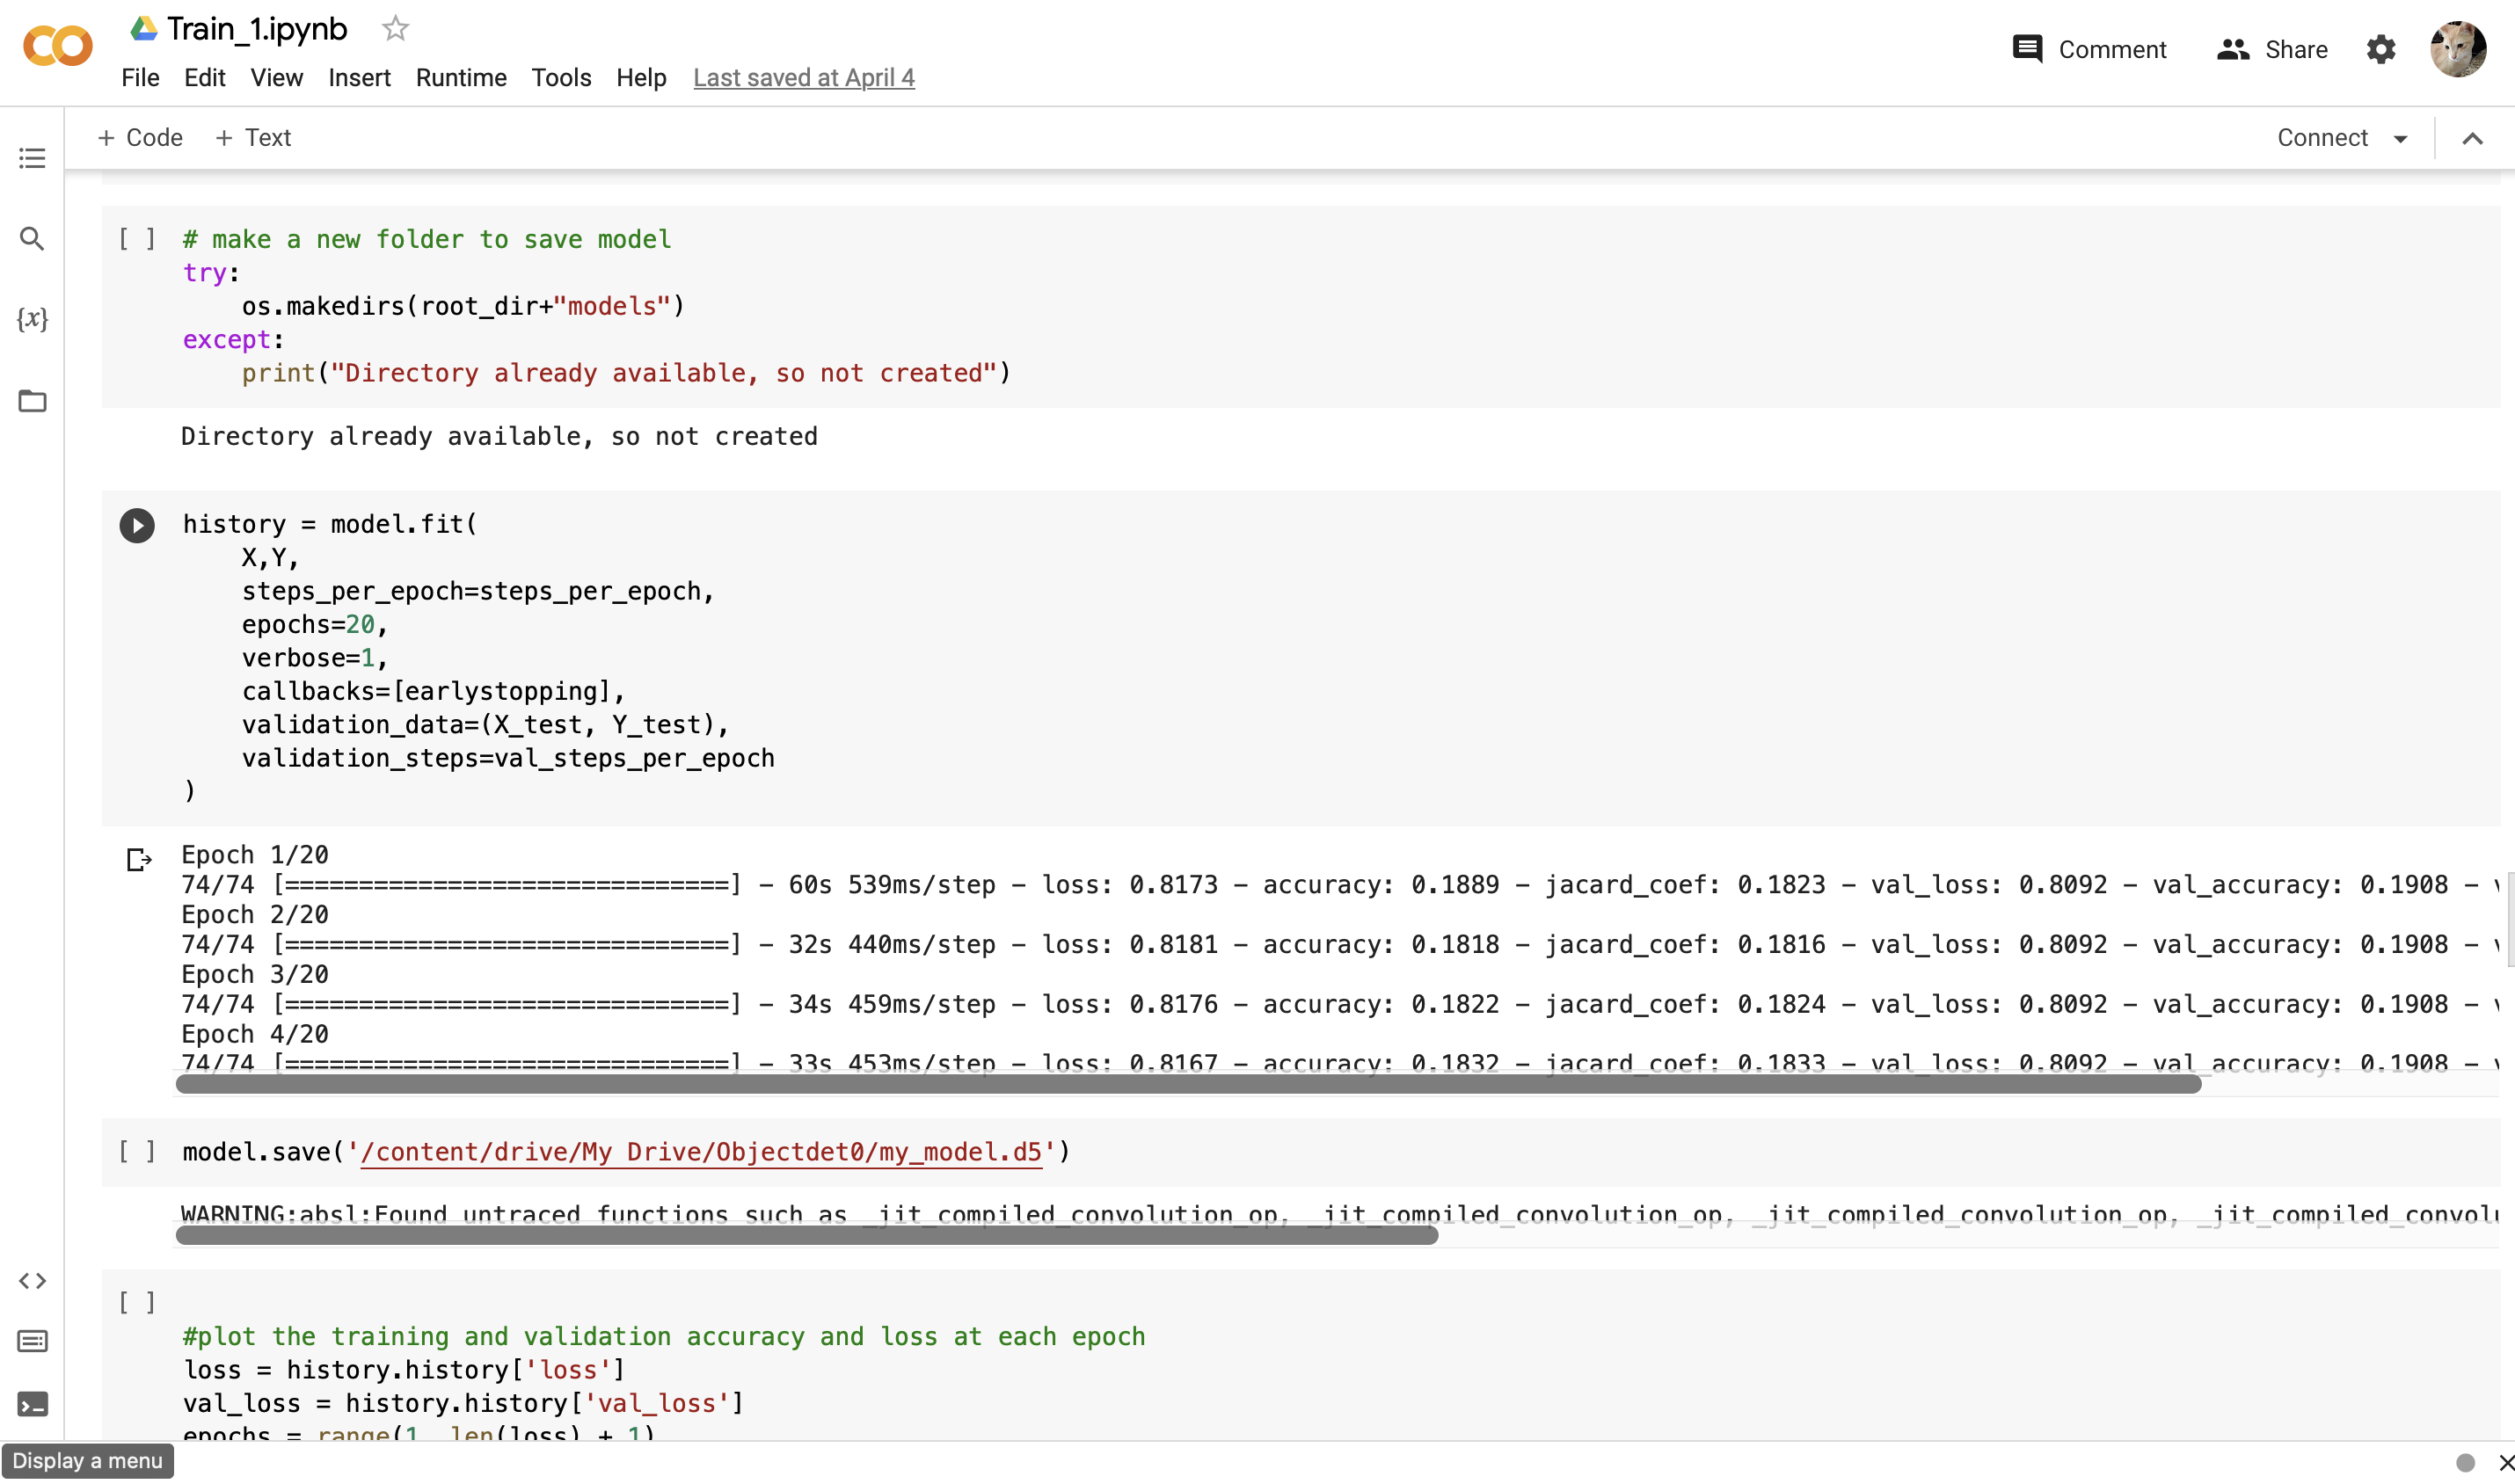
\includegraphics[scale=0.4]{screenshts/11.png}
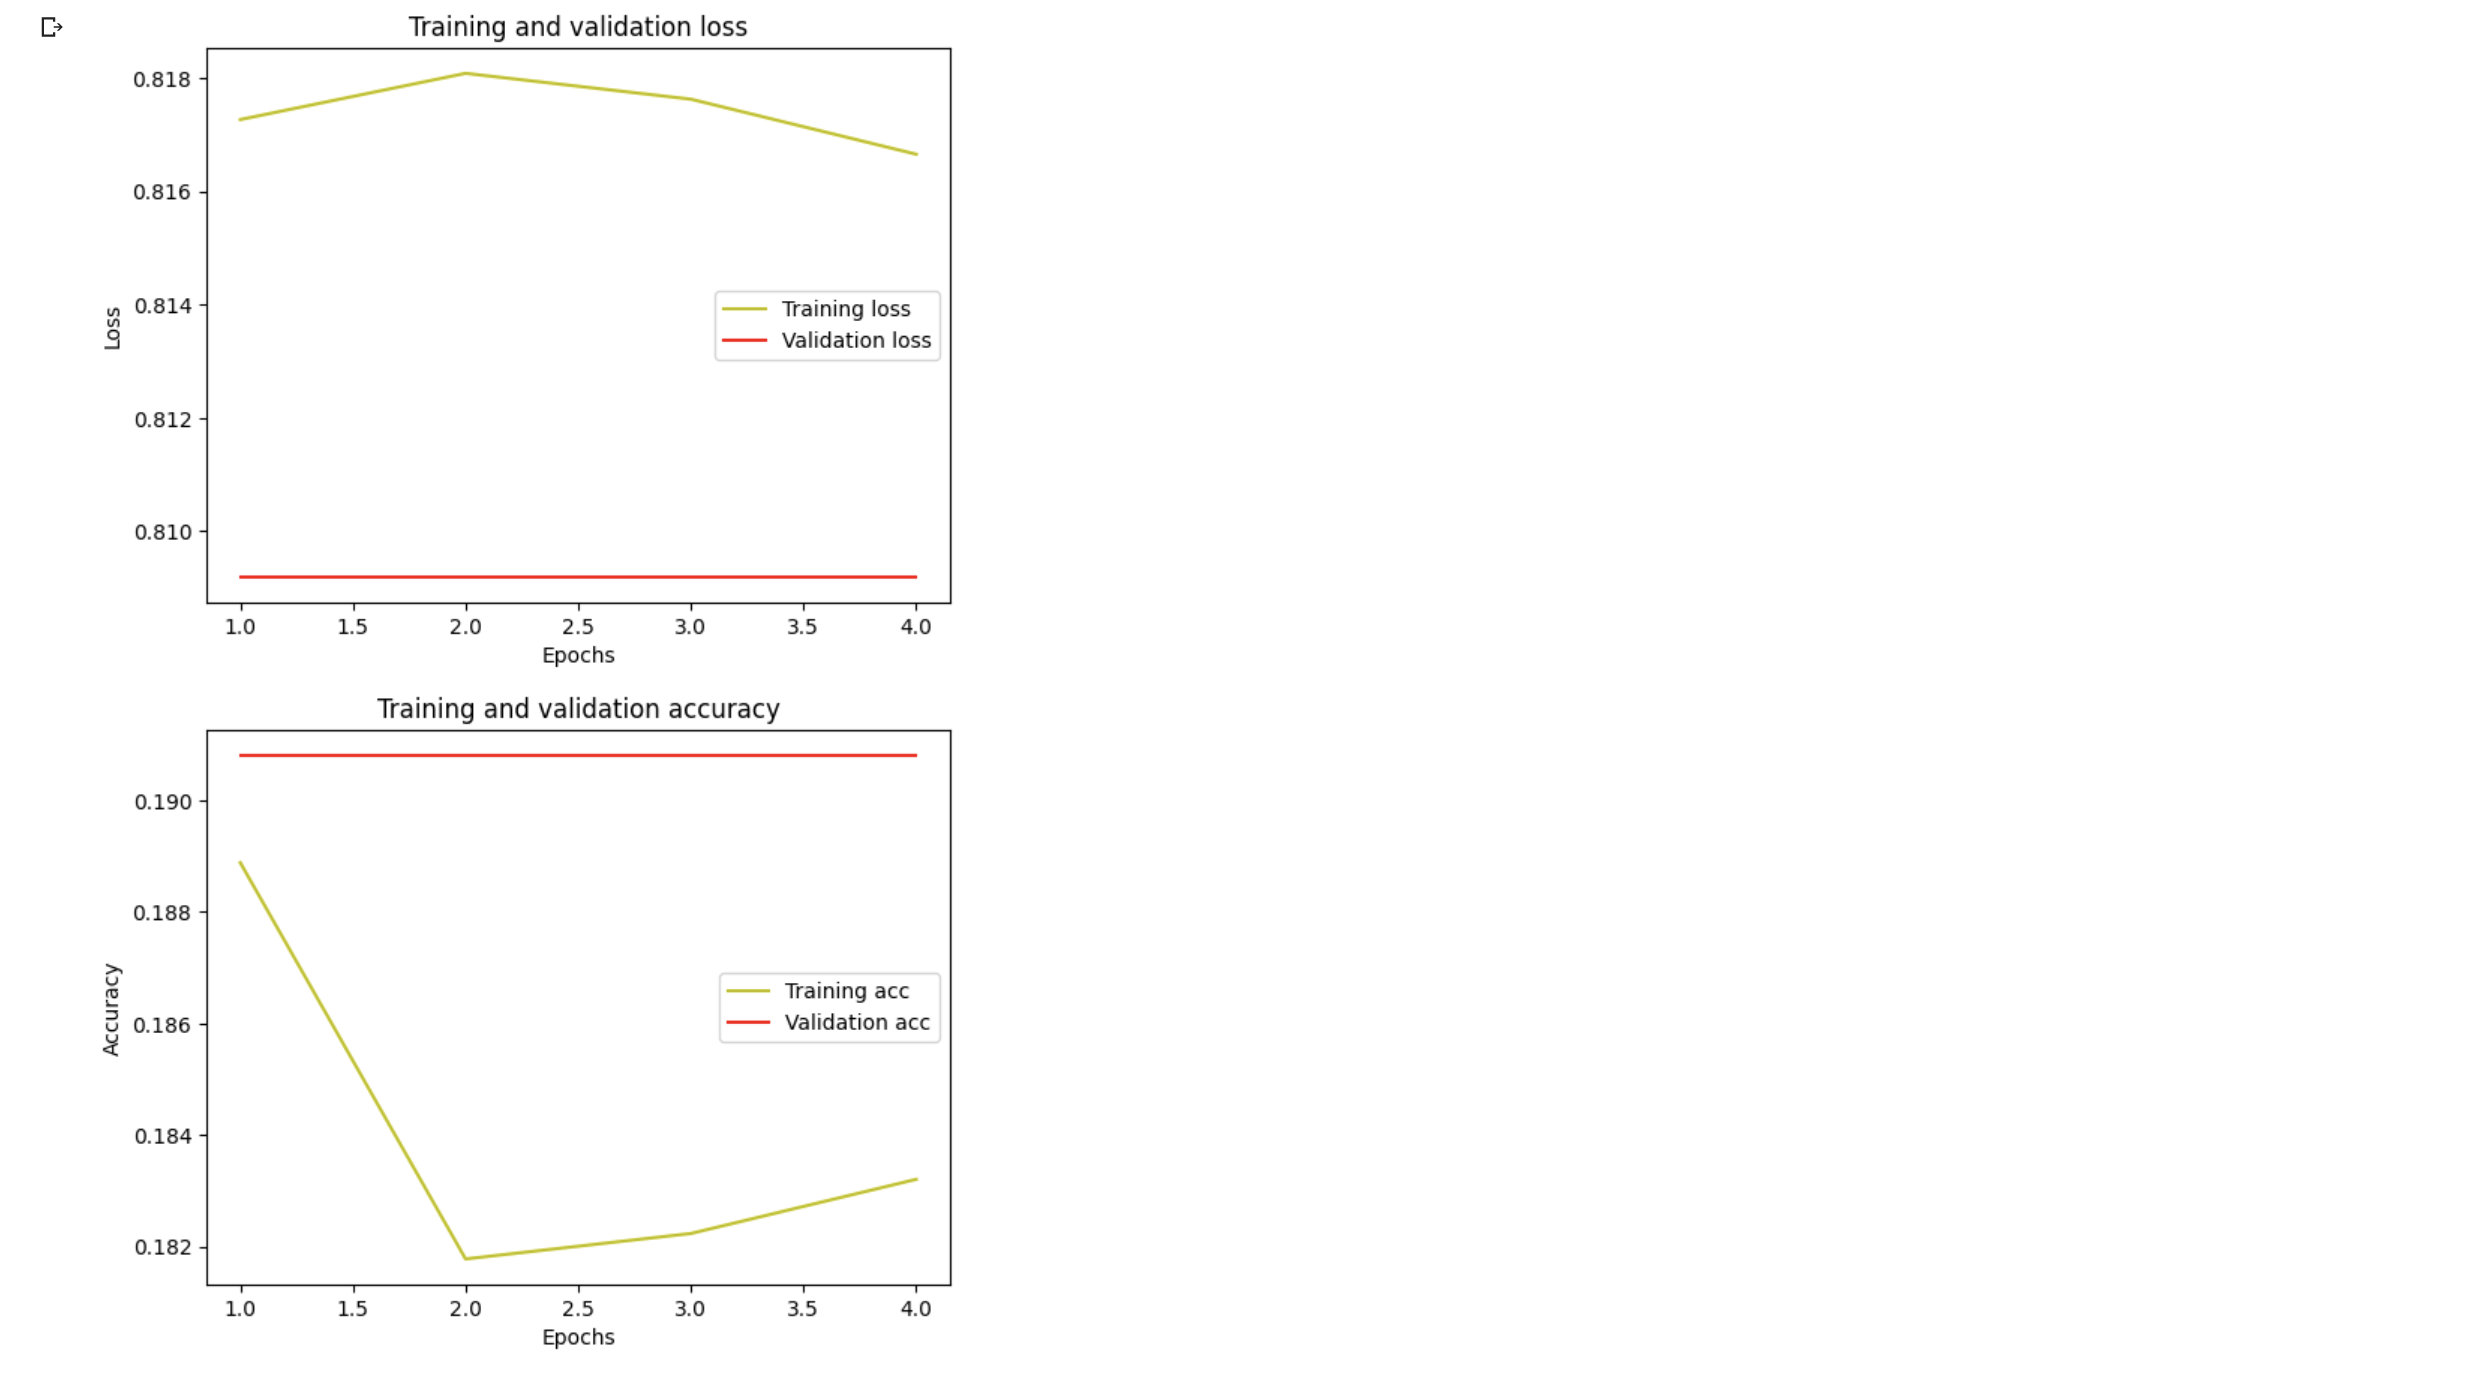
\includegraphics[scale=0.4]{screenshts/12.png}
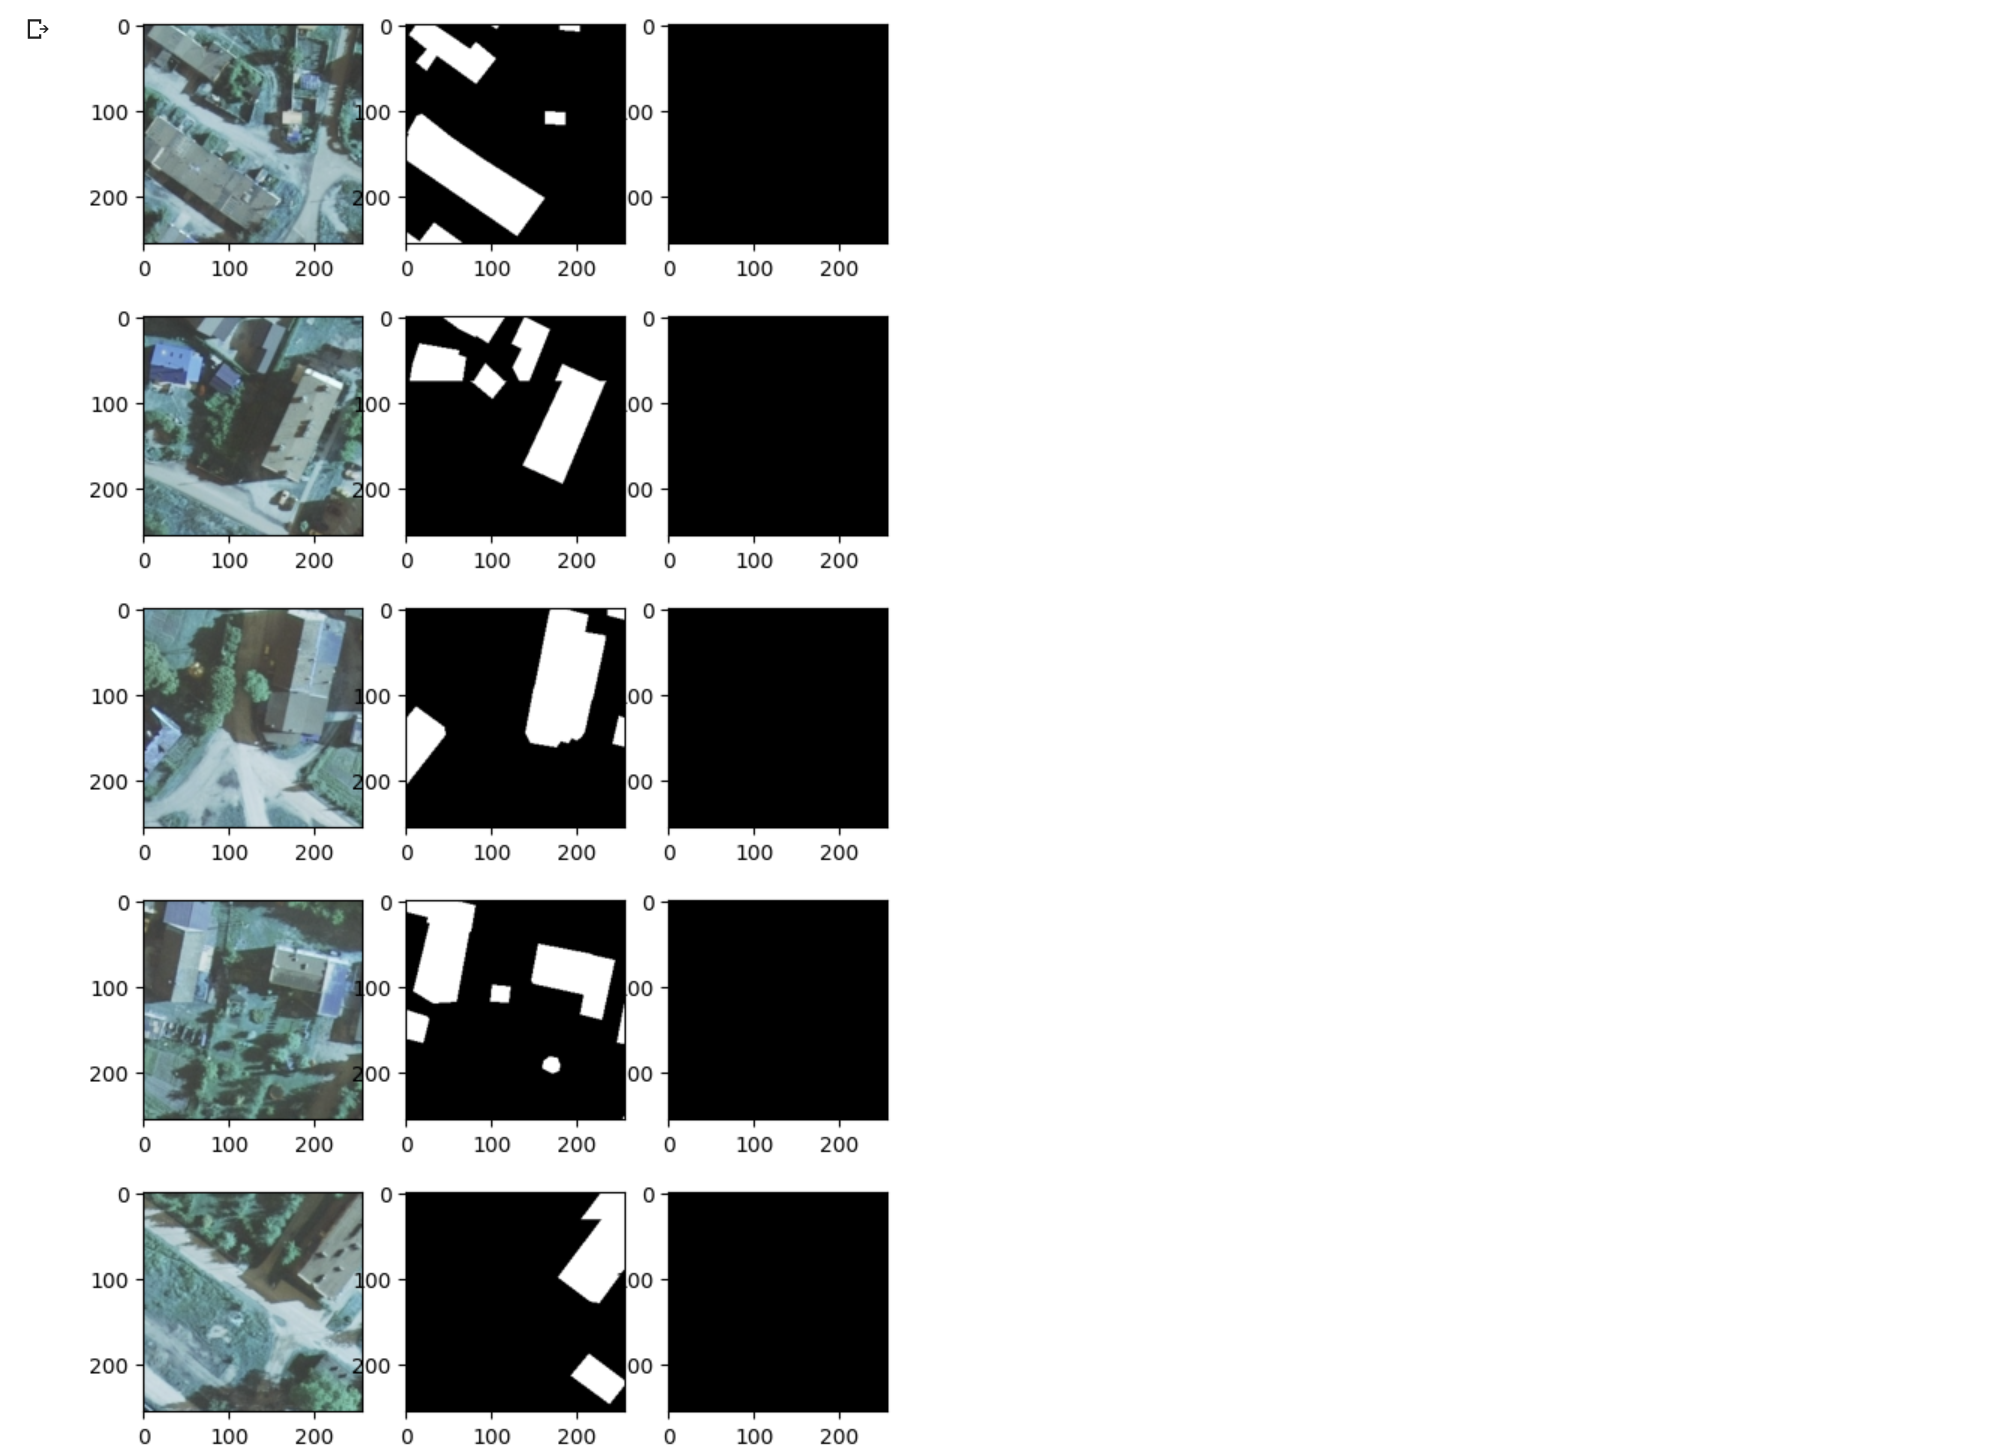
\includegraphics[scale=0.6]{screenshts/13.png}

\section{Connection to GCP Cloud using key.json}
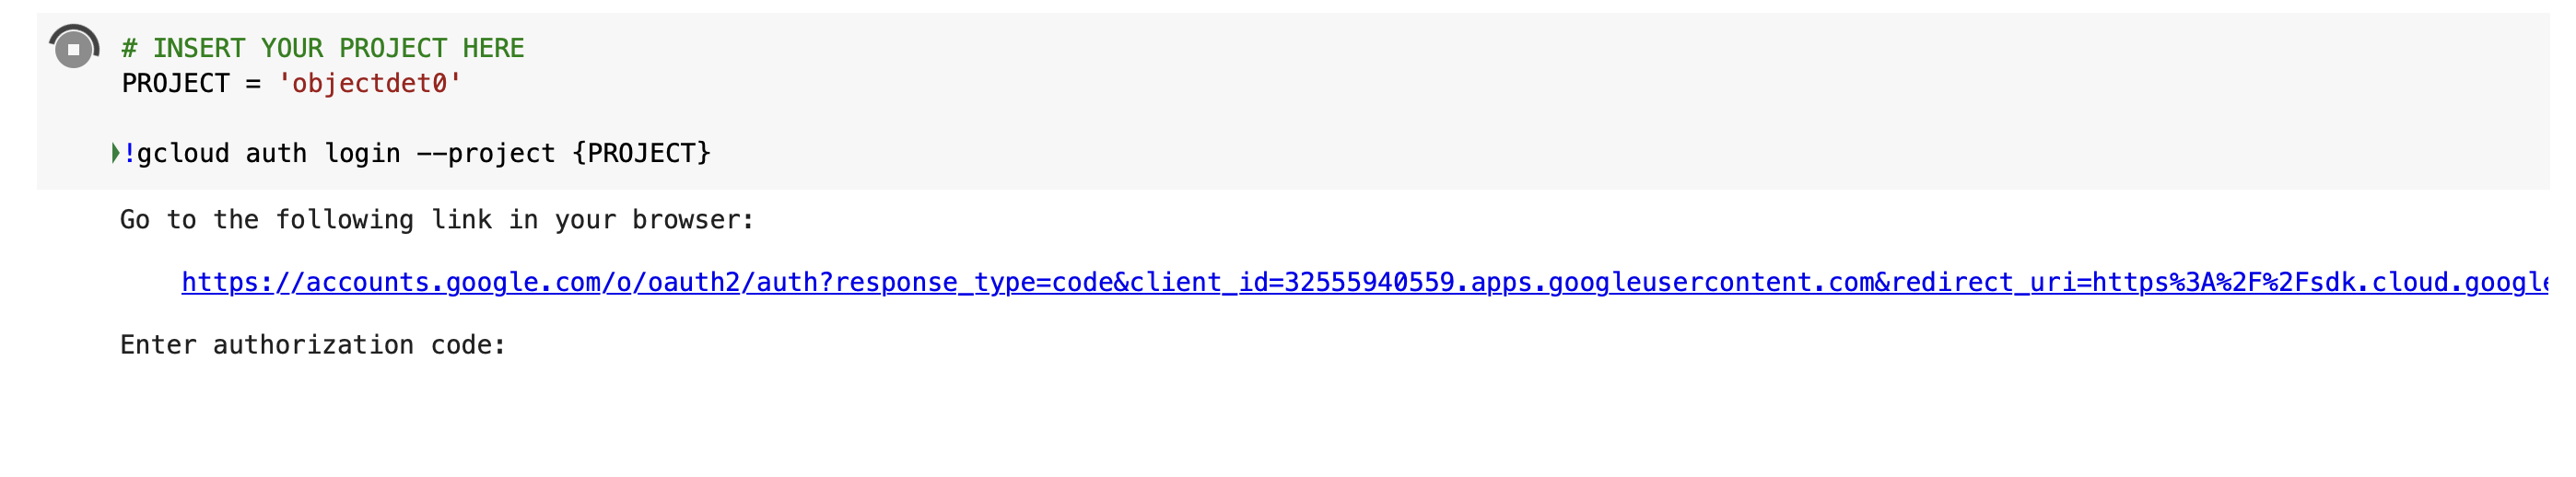
\includegraphics[scale=0.4]{screenshts/14.png}
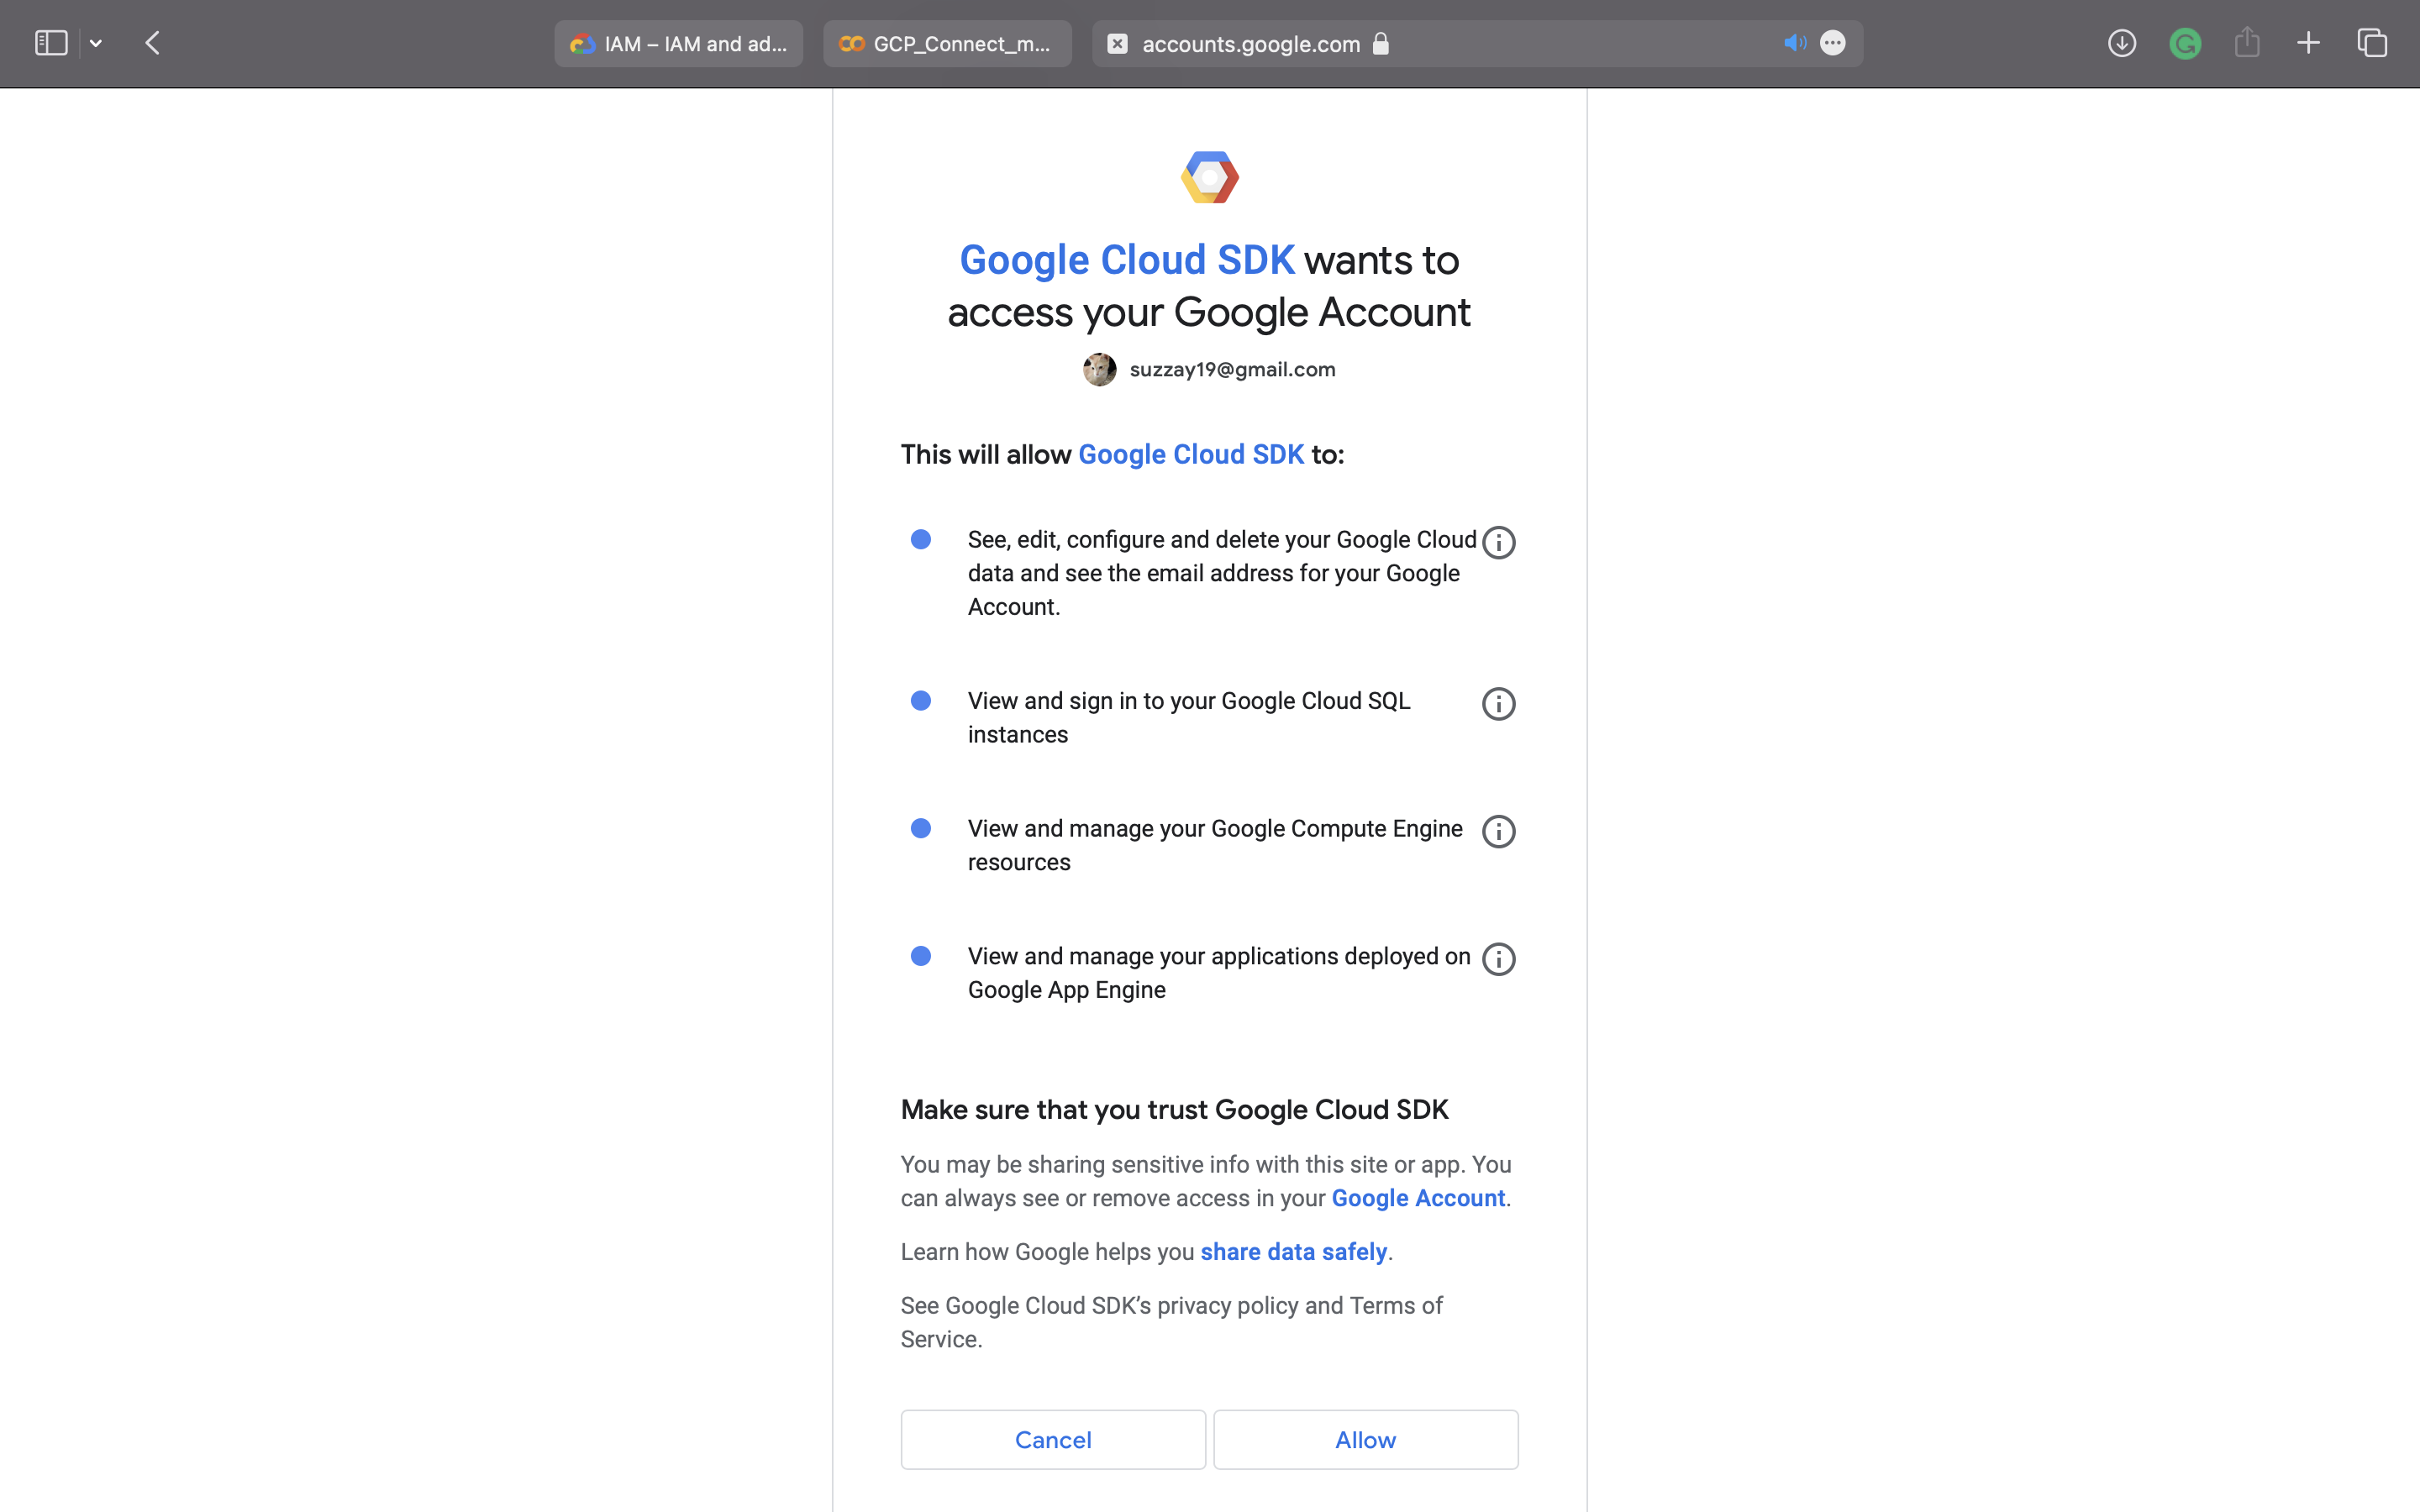
\includegraphics[scale=0.4]{screenshts/15.png}
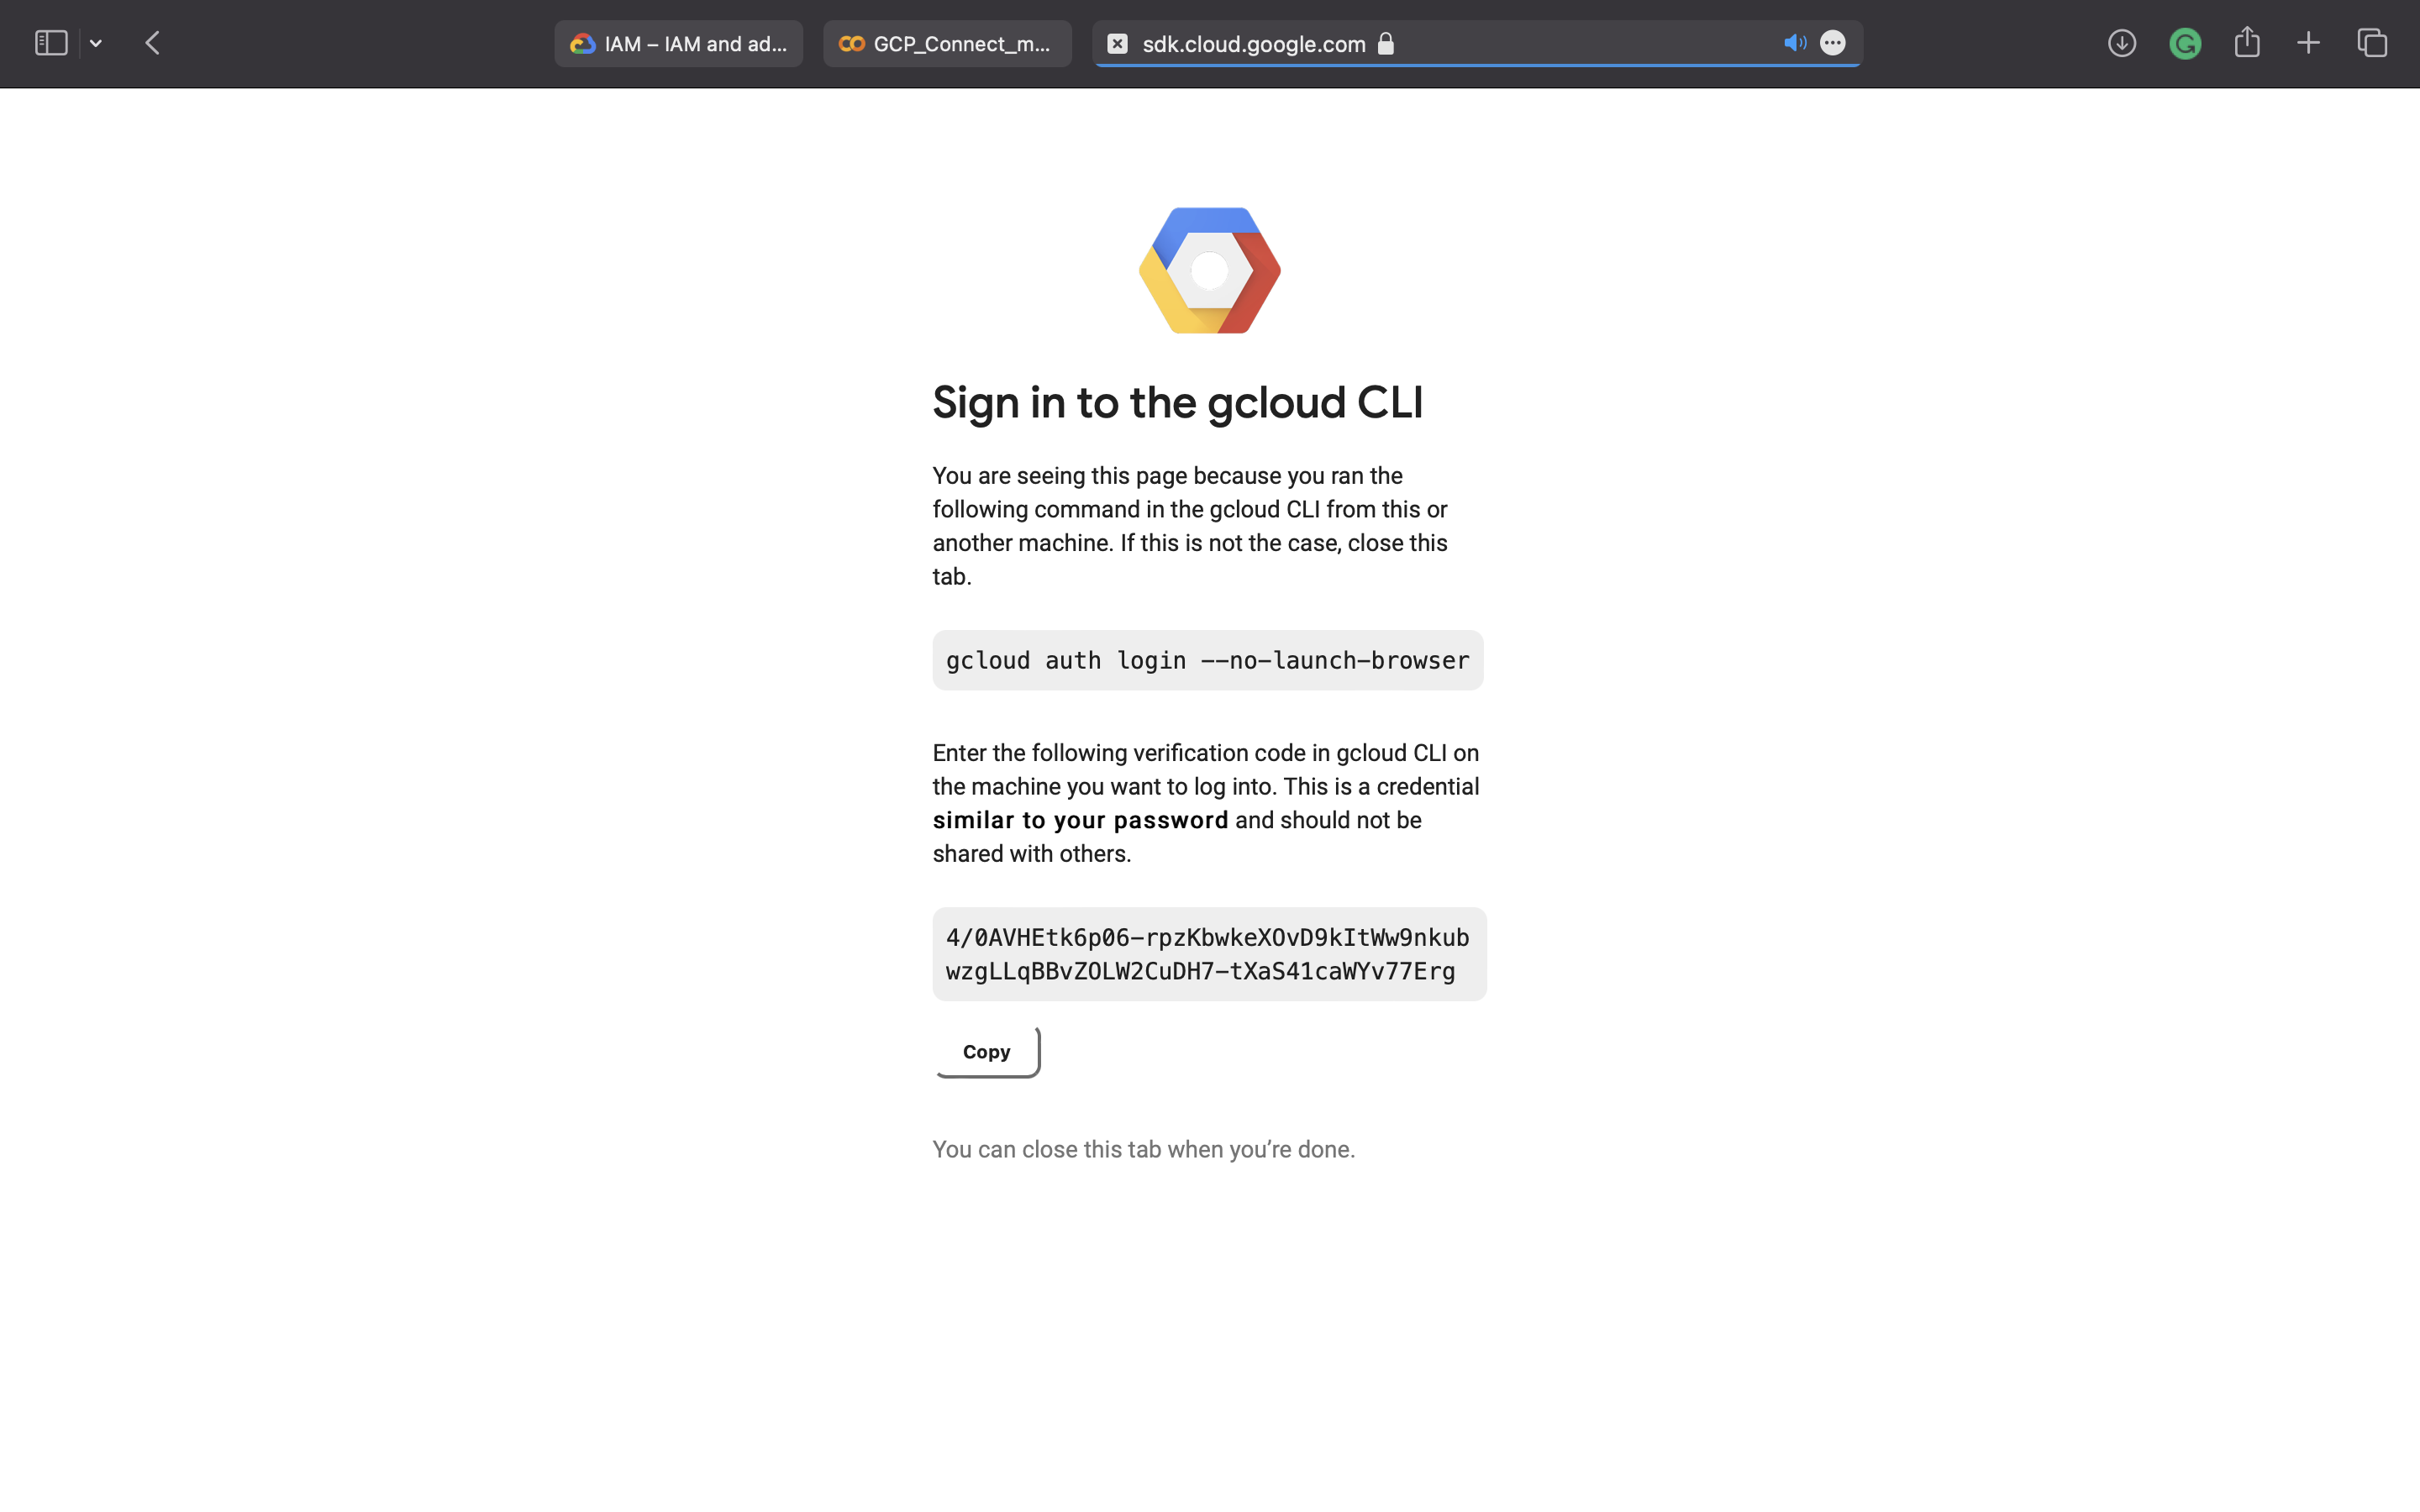
\includegraphics[scale=0.4]{screenshts/16.png}
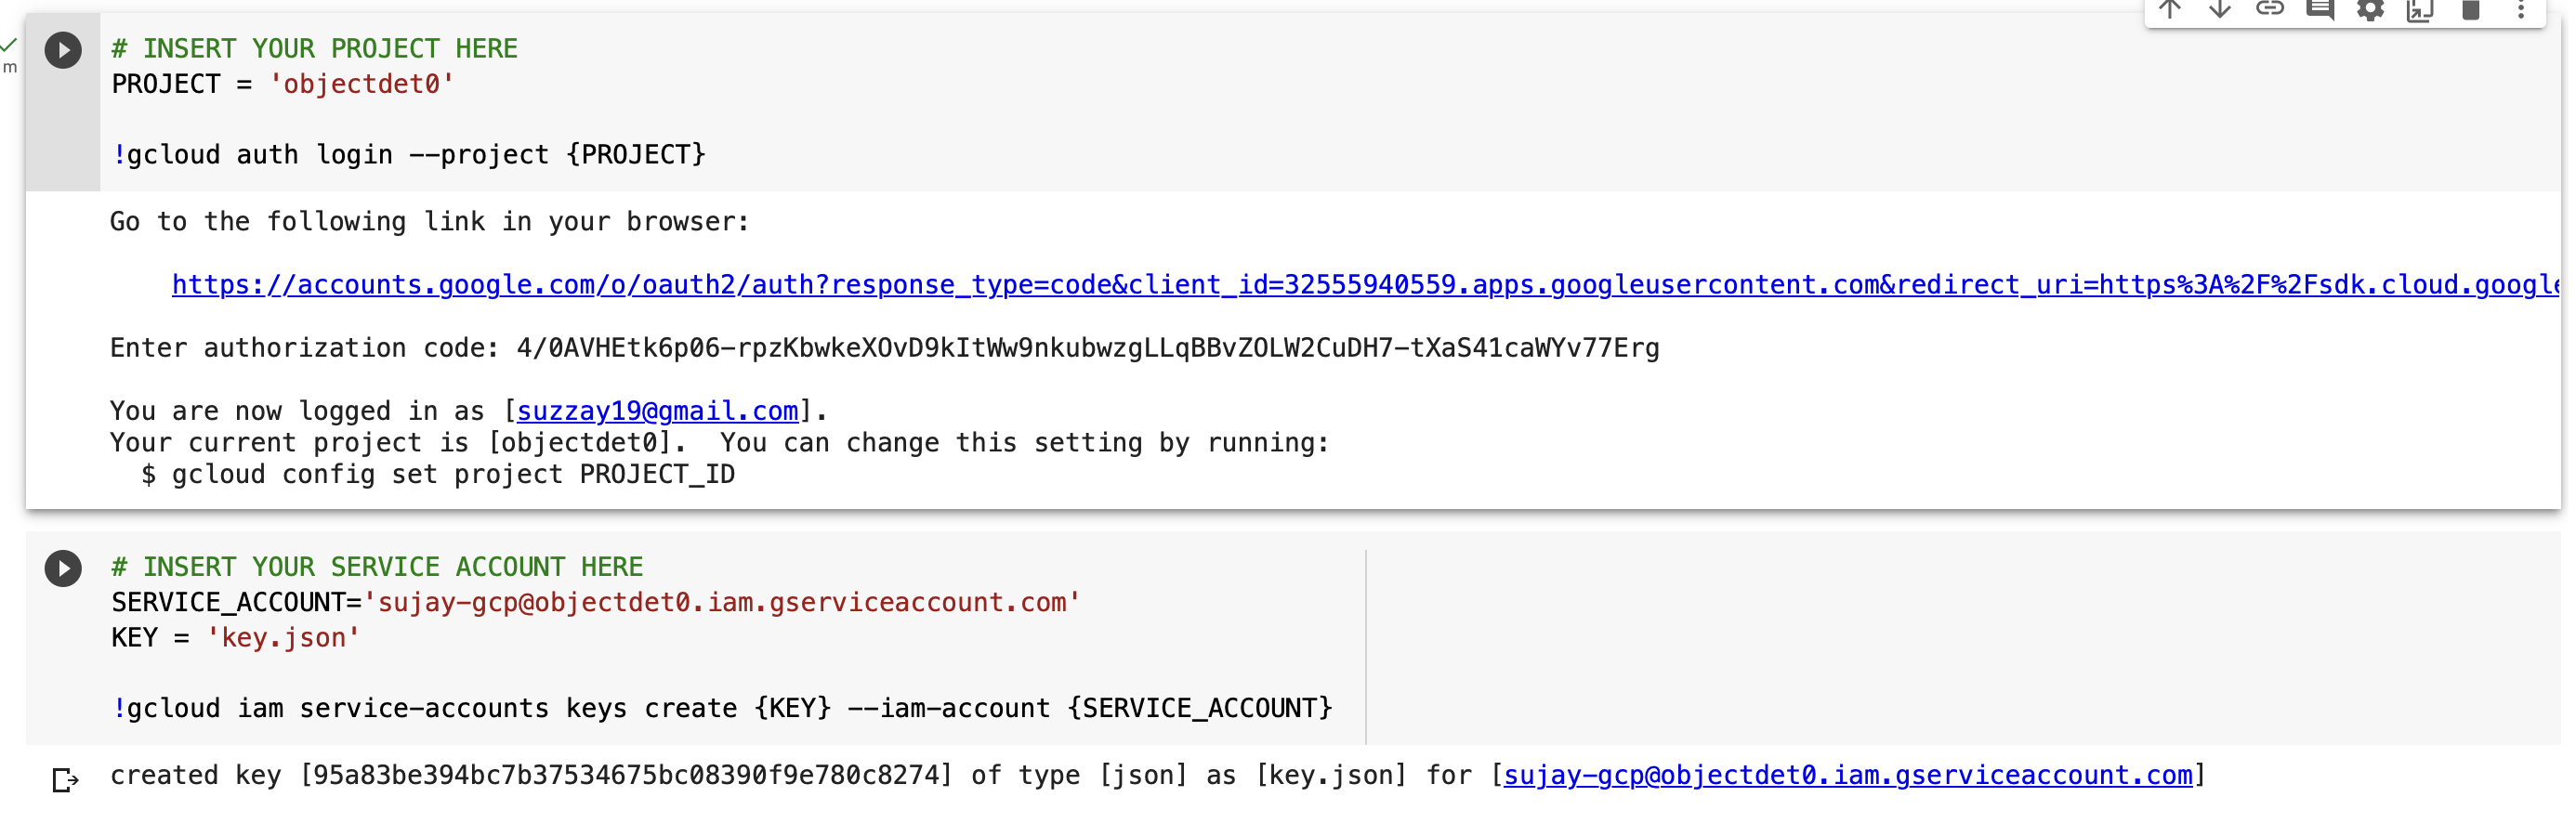
\includegraphics[scale=0.4]{screenshts/17.png}
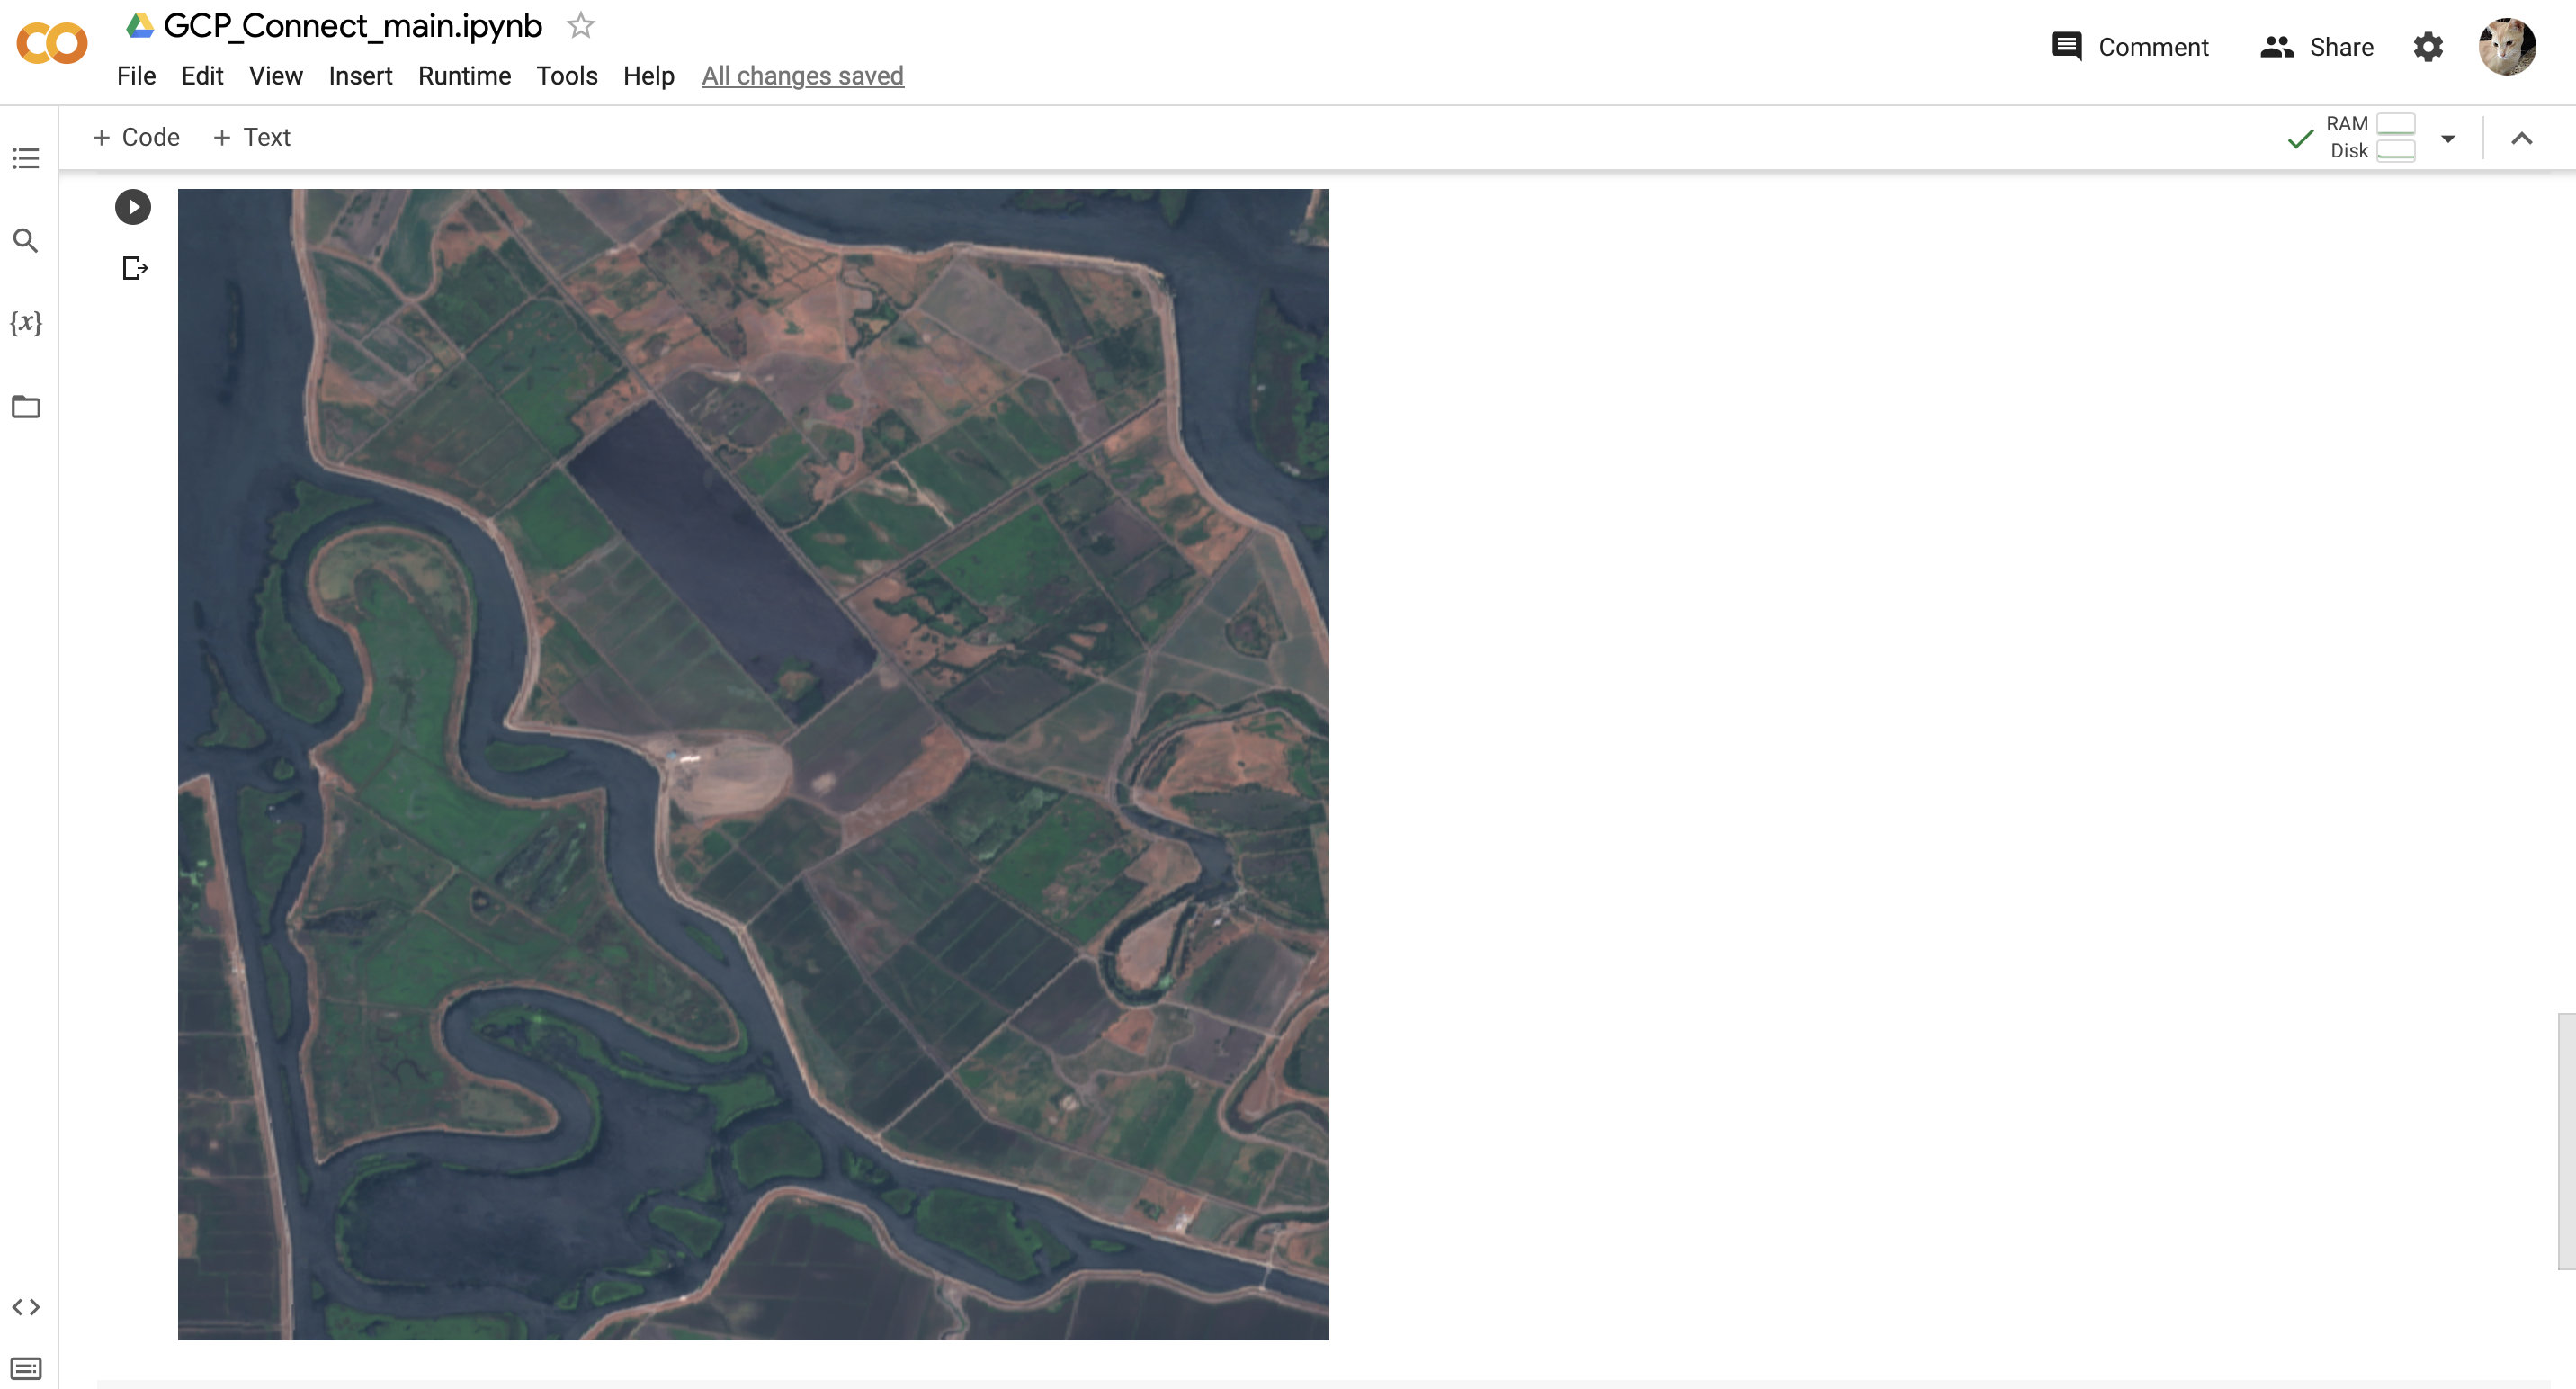
\includegraphics[scale=0.4]{screenshts/18.png}